\documentclass{article}[11pt]

\usepackage{natbib}
\usepackage[sc]{mathpazo}
\usepackage[T1]{fontenc}
\usepackage{amsmath}
\usepackage{amsfonts}
\usepackage{amssymb}
\usepackage{graphicx}
\usepackage[onehalfspacing]{setspace}
\usepackage{color}
\usepackage[margin=.75in, tmargin=0.71in, bmargin=0.71in]{geometry}
\usepackage{url}

\usepackage{chngcntr}
\usepackage{appendix}
\usepackage{hyperref}
\usepackage{xcolor}
\usepackage{todonotes}
\usepackage{booktabs}
\usepackage{lscape}
\usepackage{caption}%
\usepackage{bbm}
\usepackage{comment}

\usepackage{blindtext}

\usepackage{longtable}

\usepackage{subcaption}

\usepackage{bookmark}

\usepackage{babel}
\usepackage[autostyle, english = american]{csquotes}
\MakeOuterQuote{"}

% Centered fixed width column type
\usepackage{array}
\newcolumntype{x}[1]{>{\centering\let\newline\\\arraybackslash\hspace{0pt}}m{#1}}

\title{Textual Analysis and Financial Statements}
\author{Isaac Liu with Owen Lin, Chengzheng Xing, and Sean Zhou}

\setlength{\parindent}{0pt}
\setlength{\parskip}{0.5em}

\hypersetup{
    colorlinks=true,
    linkcolor=black,
    filecolor=black,      
    urlcolor=blue,
    citecolor=black
}

% stattotex commands
\newcommand{\avgCompanyMentions}{97.78}
\renewcommand{\avgCompanyMentions}{98.66}
\renewcommand{\avgCompanyMentions}{98.66}


\newcommand{\noCallsWithNonSelfMentions}{1884}
\newcommand{\shareCallsWithNonSelfMentions}{34.2\%}
\renewcommand{\noCallsWithNonSelfMentions}{1884}
\renewcommand{\shareCallsWithNonSelfMentions}{34.2\%}
\renewcommand{\noCallsWithNonSelfMentions}{1884}
\renewcommand{\shareCallsWithNonSelfMentions}{34.2\%}
\renewcommand{\noCallsWithNonSelfMentions}{1884}
\renewcommand{\shareCallsWithNonSelfMentions}{34.2\%}
\renewcommand{\noCallsWithNonSelfMentions}{1884}
\renewcommand{\shareCallsWithNonSelfMentions}{34.2\%}
\renewcommand{\noCallsWithNonSelfMentions}{1884}
\renewcommand{\shareCallsWithNonSelfMentions}{34.2\%}
\renewcommand{\noCallsWithNonSelfMentions}{1884}
\renewcommand{\shareCallsWithNonSelfMentions}{34.2\%}
\renewcommand{\noCallsWithNonSelfMentions}{1,884}
\renewcommand{\noCallsWithNonSelfMentions}{1884}
\renewcommand{\shareCallsWithNonSelfMentions}{34.2\%}
\renewcommand{\noCallsWithNonSelfMentions}{1,884}
\renewcommand{\shareCallsWithNonSelfMentions}{34.2\%}
\renewcommand{\noCallsWithNonSelfMentions}{1,884}
\renewcommand{\shareCallsWithNonSelfMentions}{34.2\%}
\renewcommand{\noCallsWithNonSelfMentions}{1,884}
\renewcommand{\shareCallsWithNonSelfMentions}{34.2\%}


\newcommand{\numQuarters}{4724}
\newcommand{\numCompanies}{387}
\renewcommand{\numQuarters}{4724}
\renewcommand{\numCompanies}{387}
\renewcommand{\numQuarters}{4724}
\renewcommand{\numCompanies}{387}
\renewcommand{\numQuarters}{4724}
\renewcommand{\numCompanies}{387}
\renewcommand{\numQuarters}{4724}
\renewcommand{\numCompanies}{387}
\renewcommand{\numQuarters}{4724}
\renewcommand{\numCompanies}{387}
\renewcommand{\numQuarters}{4724}
\renewcommand{\numCompanies}{387}
\renewcommand{\numQuarters}{4724}
\renewcommand{\numCompanies}{387}
\renewcommand{\numQuarters}{4724}
\renewcommand{\numCompanies}{387}
\renewcommand{\numQuarters}{4724}
\renewcommand{\numCompanies}{387}
\renewcommand{\numQuarters}{4724}
\renewcommand{\numCompanies}{387}
\renewcommand{\numQuarters}{4724}
\renewcommand{\numCompanies}{387}
\renewcommand{\numQuarters}{4724}
\renewcommand{\numCompanies}{387}
\renewcommand{\numQuarters}{4724}
\renewcommand{\numCompanies}{387}
\renewcommand{\numQuarters}{4724}
\renewcommand{\numCompanies}{387}
\renewcommand{\numQuarters}{4,724}
\renewcommand{\numCompanies}{387}
\renewcommand{\numQuarters}{4,724}
\renewcommand{\numCompanies}{387}
\renewcommand{\numQuarters}{4,724}
\renewcommand{\numCompanies}{387}

\newcommand{\avgCallLength}{8,776.18}
\renewcommand{\avgCallLength}{8,754.25}
\renewcommand{\avgCallLength}{8,754.25}
\renewcommand{\avgCallLength}{8,759.68}
\renewcommand{\avgCallLength}{8,759.68}


\newcommand{\shareNotChanges}{0.9358594411515665}
\renewcommand{\shareNotChanges}{0.9358594411515665}
\renewcommand{\shareNotChanges}{0.9358594411515665}
\renewcommand{\shareNotChanges}{93.59\%}
\renewcommand{\shareNotChanges}{93.59\%}
\renewcommand{\shareNotChanges}{93.59\%}
\renewcommand{\shareNotChanges}{93.59\%}
\renewcommand{\shareNotChanges}{94.66\%}
\renewcommand{\shareNotChanges}{94.66\%}
\renewcommand{\shareNotChanges}{94.66\%}
\renewcommand{\shareNotChanges}{94.66\%}
\renewcommand{\shareNotChanges}{94.66\%}
\renewcommand{\shareNotChanges}{94.66\%}
\renewcommand{\shareNotChanges}{94.66\%}
\renewcommand{\shareNotChanges}{94.66\%}


\newcommand{\rNeg}{39}
\renewcommand{\rNeg}{39}
\newcommand{\rPosScoreFinbert}{42}
\renewcommand{\rNeg}{39}
\renewcommand{\rPosScoreFinbert}{42}
\newcommand{\rNumTransparency}{68}
\newcommand{\rWordCount}{135}
\newcommand{\rGfScore}{122}
\renewcommand{\rNeg}{39}
\renewcommand{\rPosScoreFinbert}{42}
\newcommand{\rUndrst}{52}
\renewcommand{\rNumTransparency}{68}
\renewcommand{\rWordCount}{135}
\renewcommand{\rGfScore}{122}


\newcommand{\numTrainNodes}{1562}
\newcommand{\numTestNodes}{402}
\newcommand{\numNodes}{1964}
\newcommand{\averageDegree}{1.7993890020366599}
\newcommand{\numEdges}{1806}
\renewcommand{\numTrainNodes}{1562}
\renewcommand{\numTestNodes}{402}
\renewcommand{\numNodes}{1964}
\renewcommand{\averageDegree}{1.8}
\renewcommand{\numEdges}{1806}
\renewcommand{\numTrainNodes}{1,562}
\renewcommand{\numTestNodes}{402}
\renewcommand{\numNodes}{1,964}
\renewcommand{\averageDegree}{1.8}
\renewcommand{\numEdges}{1,806}


\newcommand{\retrainLRAccuracy}{0.6244}
\newcommand{\retrainXGBAccuracy}{0.8209}
\newcommand{\pretrainedLRAccuracy}{0.6692}
\newcommand{\pretrainedXGBAccuracy}{0.893}
\renewcommand{\retrainLRAccuracy}{0.6244}
\renewcommand{\retrainXGBAccuracy}{0.8209}
\renewcommand{\pretrainedLRAccuracy}{0.6692}
\renewcommand{\pretrainedXGBAccuracy}{0.893}
\renewcommand{\retrainLRAccuracy}{0.6219}
\renewcommand{\retrainXGBAccuracy}{0.8209}
\renewcommand{\pretrainedLRAccuracy}{0.6692}
\renewcommand{\pretrainedXGBAccuracy}{0.893}
\renewcommand{\retrainLRAccuracy}{0.6219}
\renewcommand{\retrainXGBAccuracy}{0.8209}
\renewcommand{\pretrainedLRAccuracy}{0.6692}
\renewcommand{\pretrainedXGBAccuracy}{0.893}
\renewcommand{\retrainLRAccuracy}{0.6234}
\renewcommand{\retrainXGBAccuracy}{0.8229}
\renewcommand{\pretrainedLRAccuracy}{0.6683}
\renewcommand{\pretrainedXGBAccuracy}{0.8928}
\renewcommand{\retrainLRAccuracy}{0.6234}
\renewcommand{\retrainXGBAccuracy}{0.8229}
\renewcommand{\pretrainedLRAccuracy}{0.6683}
\renewcommand{\pretrainedXGBAccuracy}{0.8928}
\renewcommand{\retrainXGBAccuracy}{0.8229}
\renewcommand{\retrainLRAccuracy}{0.6234}
\renewcommand{\retrainXGBAccuracy}{0.8229}
\renewcommand{\pretrainedLRAccuracy}{0.6683}
\renewcommand{\pretrainedXGBAccuracy}{0.8928}


\newcommand{\ratingRGAcc}{0.2245}
\newcommand{\changeRGAcc}{0.898}
\renewcommand{\ratingRGAcc}{0.2245}
\renewcommand{\changeRGAcc}{0.898}


\newcommand{\trainCount}{4,391}
\newcommand{\testCount}{1,118}
\renewcommand{\trainCount}{4,391}
\renewcommand{\testCount}{1,118}



\begin{document}

	\maketitle

    \section*{Introduction}

    Corporate credit ratings represent professional estimations of the default risk carried by company debt. These ratings represent critical information for investors - not just institutional investors and financially sophisticated bondholders, but also individual stockholders, who may be wiped out completely in the event of bankruptcy. Analyzing ways to predict ratings can offer substantial value to a variety of stakeholders. Predictive models may be useful for investors without access to data, companies or potential lenders that seek information about influential factors,\footnote{There is evidence suggesting financial factors and projections have a causal impact on ratings and are not manipulated by companies in response to forecasted rating changes \citep{he_impact_2018}.} and by any parties seeking interpolated ratings for companies that do not have them.

    In this project, we seek to fully leverage the text of earnings calls, along with traditional financial measures and variables, to improve predictions of corporate credit ratings for any given company and quarter and better understand the importance of various influences.\footnote{Though much literature has focused on financial statements and reports and credit ratings (as just one example, see \cite{makwana_understanding_2022}), our paper takes a relatively underexplored approach, instead incorporating earnings call transcripts. We believe calls offer a richer picture of a firm's financial prospects because they include two-way conversation between company management and financial analysts in form of a Q and A section. This section incorporates the broader beliefs and concerns of the financial community into our predictions. Additionally, in contrast to financial statements, which must be (noisily) parsed to identify sections relevant to management analysis, earnings calls provide more directly valuable and readily available information.} Features capturing call readability, transparency, and engagement join classical and pre-trained language model representations of sentiment \citep{araci_finbert_2019} and traditional tabular variables as inputs to a variety of supervised machine learning techniques for classification from logistic regression to tree-based methods. We also make use of advances in the study of graph neural networks to model linkages between firms \citep{das_credit_2023}, in our case implied by mentions in calls.

    To the best of our knowledge, the closest prior work to ours is \cite{donovan_measuring_2021}, which leverages the textual content of earnings calls and financial statements to predict credit events such as bankruptcies, interest spread changes, and rating downgrades. Unigram and bigram word frequencies were used with the supervised machine learning techniques of Support Vector Regression, Latent Dirichlet Allocation, and Random Forests. The coefficient on a constructed textual measure of credit risk was found to be significant up to the 1\% level. In contrast to this approach, we focus on predicting the credit ratings themselves, and integrate more recent techniques such as neural language models and a wider variety of algorithms for classification.

    \section*{Data and Exploratory Data Analysis}

    We combine a wide variety of data sources to support our predictions of credit ratings - merging rating data with company earnings calls, financial statement variables, and industry sector. In our combined dataset, each observation represents a fixed quarter date (1/1, 4/1, 7/1, 10/1) for a company, with the company's most recent credit rating, earnings call and associated financial statement variables, and sector attached. An example of many of the variables for a company by fixed quarter date can be found in Appendix Section \ref{sec:one-obs-final-data}.

    Our scope of interest is publicly traded companies from 2010-2016 (a limitation due to the availability of credit rating data) - the distribution of call year and quarters can be found in Appendix Figure \ref{fig:obs-by-quarter-year}. We took many steps to remove or Winsorize errors and outliers - details of our data cleaning and filtering steps can be found in Appendix Section \ref{sec:data-cleaning}. In all, we have \numQuarters \space quarters for \numCompanies \space unique companies.

    \subsection*{Credit Ratings}

    We make use of long-term credit rating issuances from S and P Rating Services, provided from a combination of two credit rating datasets downloaded in CSV and Excel format from Kaggle \citep{gewerc_corporate_2020,makwana_corporate_2022}. Each issuance can be a change in rating (upgrade, downgrade) or reaffirmation - they occur at ad-hoc intervals. We reshape these rating issuances to a dataset of ratings for each company on each fixed quarter date by creating a rating end date variable that is the date of the next issuance or end of data, and joining a list of the fixed quarter dates on the condition that the fixed quarter date is between the issuance date and the end date.

    Figure \ref{fig:credit-ratings} shows the distribution of rating grades used in our final dataset. Finer grades (AA+, CCC-, etc.) are sometimes assigned by agencies, but these grades were converted by dropping the +/- for this project. Ratings of BBB and above are considered investment grade - these bonds carry empirical one-year default rates of 0 to 1\%. Ratings below that are classified as junk, with default rates from 1 to 30, 40, or even 50\% for some years \citep{s_and_p_global_ratings_s_2024}. Most company-quarters have ratings around the BBB threshold, with very few cases on the extreme ends of the spectrum. Ratings also tend to be constant over time. Relative to the previous fixed quarter date, \shareNotChanges \space of ratings remain the same. When available, rating on the previous fixed quarter date can thus be an extremely strong predictor.

    \begin{figure*}
        \caption{Credit Ratings}
        \begin{subfigure}[h]{0.4925\textwidth}
            \centering
            \subcaption{Distribution}
            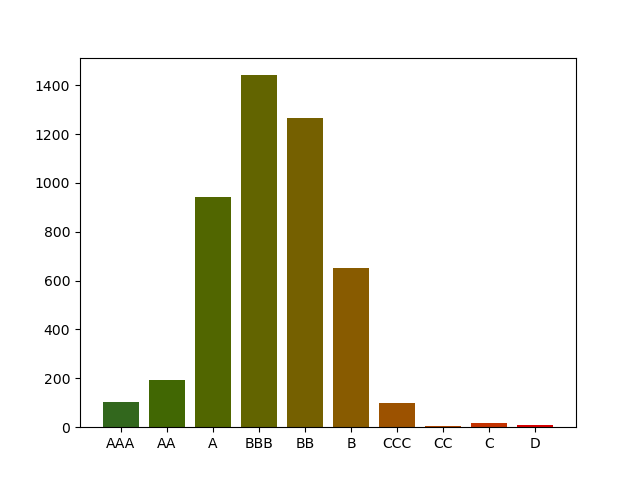
\includegraphics[width=0.95\hsize]{../Output/All Data EDA/Tabular EDA/Distribution of Rating Issuances_no_title.png}
        \end{subfigure}
        %\hfill
        \begin{subfigure}[h]{0.4925\textwidth}
            \centering
            \subcaption{Change Between Fixed Quarter Dates}
            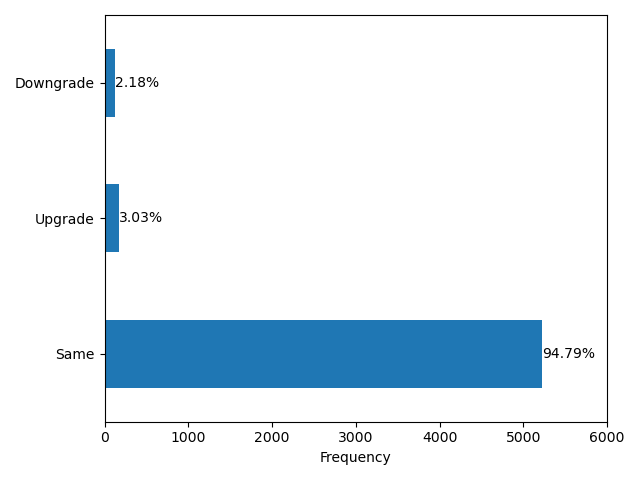
\includegraphics[width=0.95\hsize]{../Output/All Data EDA/Tabular EDA/Change_Short_no_title.png}
        \end{subfigure}
        \hfill
        \label{fig:credit-ratings}
    \end{figure*}

    \subsection*{Earnings Calls}

    Our earnings call data comes from the Financial Modelling Prep API \citep{financial_modeling_prep_financial_2024}, a trusted source widely used in industry. Including both prepared remarks and analyst Q and A sessions, the overall average call length in our final data stands at \avgCallLength \space words.

    \subsection*{Financial Statements}

    Our financial statement variables are also retrieved using the Financial Modelling Prep API. We make use of items from company balance sheets, cash flow statements, and income statements, as well as company market capitalization. We also calculated and included a wide variety of ratios and combinations of levels of variables (for a list, see Appendix Section \ref{sec:financial-summary-statistics}).

    \begin{figure*}
        \caption{Altman Z-Score}
        \begin{subfigure}[h]{0.4925\textwidth}
            \centering
            \subcaption{Distribution}
            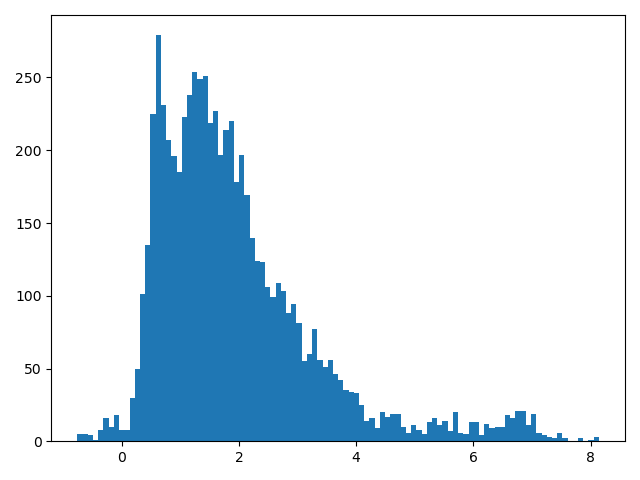
\includegraphics[width=0.95\hsize]{../Output/All Data EDA/Tabular EDA/altman_z_score_all_data_no_title.png}
        \end{subfigure}
        %\hfill
        \begin{subfigure}[h]{0.4925\textwidth}
            \centering
            \subcaption{Average by Rating}
            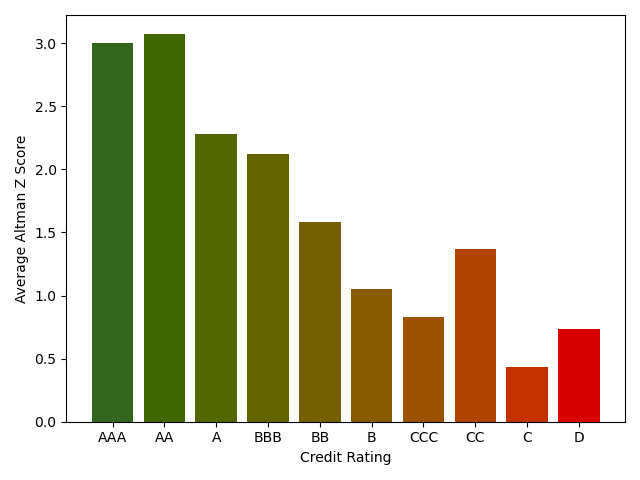
\includegraphics[width=0.95\hsize]{../Output/All Data EDA/Tabular EDA/mean_altman_Z_by_credit_rating_no_title.png}
        \end{subfigure}
        \hfill
        \label{fig:altman-z-score}
    \end{figure*}

    In some of our models, we make use of Altman's Z-score \citep{altman_financial_1968}, a traditional measure of bankruptcy risk that accounts for company earnings, equity, and assets and liabilities (for details on the construction of the score, see Appendix Section \ref{sec:altman-z-score}). Figure \ref{fig:altman-z-score} shows the distribution of Z-scores in our dataset. Traditionally, values above 3.0 have been considered safe, while those below 1.8 are considered to imply a high chance of bankruptcy.  The average scores for each rating in our data seem to align well with this interpretation, with high scores being associated with higher ratings in a linear manner. Though our distribution of scores is skewed, with a long right tail, and though the relationship between ratings and average scores breaks down on the ends of the rating spectrum (where not many companies and ratings are available), Z-Score demonstrated potential as a predictor.
      
    \subsection*{Sector}

    The GCIS industry classification standard divides companies into 11 major industry sectors \citep{s_and_p_gics_2024}.\footnote{There are finer groupings as well, but this data was not easily obtainable for our project.} It is widely used in the financial community, and was developed in part by S and P, the same company responsible for our credit ratings. We obtained classifications from Kaggle in CSV format \citep{kozlov_us_2022} and supplemented them with manual lookup. Figure \ref{fig:firms-by-sector} shows the sectoral imbalance present in our data, with a large share of firms in consumer, industrial, and technology sectors. However, when we quantify ratings and compute average values by sector, we do not see large differences, suggesting our results still may provide some generalizability. Though it was not clear that sector alone provided enough useful variation in rating to be a useful predictor, we still included it in our models based on its potential to improve models including other controls or interactions.

    \begin{figure*}
        \caption{Sector}
        \begin{subfigure}[h]{0.4925\textwidth}
            \centering
            \subcaption{Firms by Sector}
            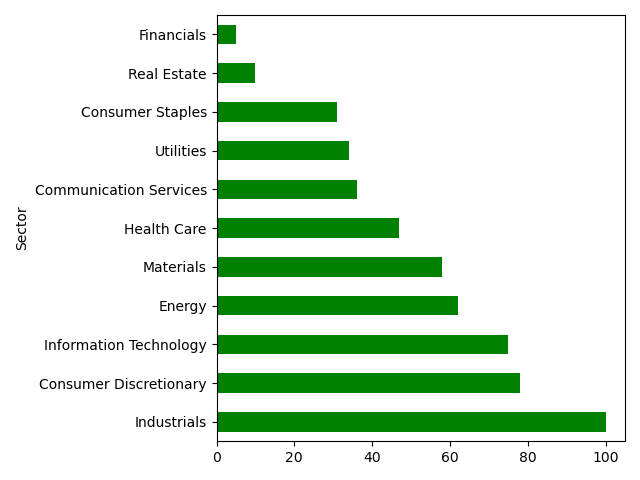
\includegraphics[width=0.95\hsize]{../Output/All Data EDA/Tabular EDA/all_data_fixed_quarter_dates_firms_by_sector_no_title.png}
        \end{subfigure}
        %\hfill
        \begin{subfigure}[h]{0.4925\textwidth}
            \centering
            \subcaption{Average Rating by Sector}
            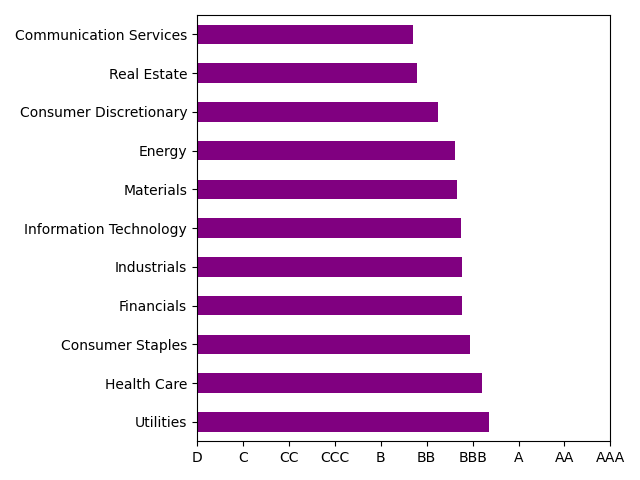
\includegraphics[width=0.95\hsize]{../Output/All Data EDA/Tabular EDA/all_data_fixed_quarter_dates_average_credit_rating_by_sector_no_title.png}
        \end{subfigure}
        \hfill
        \label{fig:firms-by-sector}
    \end{figure*}

    \section*{NLP Features}

    We make use of techniques from Natural Language Processing (NLP) to create features to capture the transparency of discussion, level of engagement, and overall sentiment of calls.

    \begin{itemize}
        \item Numeric Transparency - Ratio of numbers to words in the word-tokenized call
        \item Readability - We construct the Gunning-Fog grade-level readability score \citep{gunning_technique_1952} as 
        \begin{equation*}
            0.4 \times (\frac{\text{Words}}{\text{Sentences}} + 100 \times \frac{\text{3+ Syllable Words}}{\text{Words}})
        \end{equation*}
        \item Word Count
        \item Normalized Number of Questions - Count of question marks, divided by call word count
        \item Tone - Following \cite{price_earnings_2012}, we use the Harvard IV Psychosocial dictionary to count words falling in various categories (Positive, Negative, Active, Passive, etc.).\footnote{In addition to the tone feature described, we also incorporate these counts as individual features.} Then we construct tone using the first principal component of the matrix with each call as a row and each column as one of the following:
        \begin{equation*}
            \frac{\text{Positive}}{\text{Negative}}, \frac{\text{Active}}{\text{Passive}}, \frac{\text{Strong}}{\text{Weak}}, \frac{\text{Overstated}}{\text{Understated}}
        \end{equation*}
        \item FinBERT Positivity Score - We use FinBERT, a version of the transformer-model BERT finetuned for the financial domain to determine the tone (positive, negative, neutral) of sentences in each call.\footnote{We originally considered directly incorporating FinBERT embeddings into our models, or creating an end-to-end classifier making use of a BERT model. Our calls, however, are too long for readily available transformer embeddings or models to efficiently and effectively represent.} \citep{huang_finbert_2023} In line with \cite{kantos_comparative_2022}, we then calculate a positivity score for the call as:
        \begin{equation*}
            \text{FinBERT Positivity Score} = log_{10}\frac{\text{Count Positive} + 1}{\text{Count Negative} + 1}
        \end{equation*}
    \end{itemize}

    Examples for readability and tone can be found in Appendix Section \ref{sec:nlp-examples}, and the distribution of each NLP feature by rating is shown in Figure \ref{fig:dist-nlp-by-rating} below. Lower quality companies seem to provide more numbers with less commentary. It appears to be the case that higher quality companies tend to have longer calls. Though somewhat noisy, our FinBERT positivity score does seem to correlate with higher ratings.

    \begin{figure}[h!]
		\centering
        \caption{Distribution of NLP Features by Rating}
        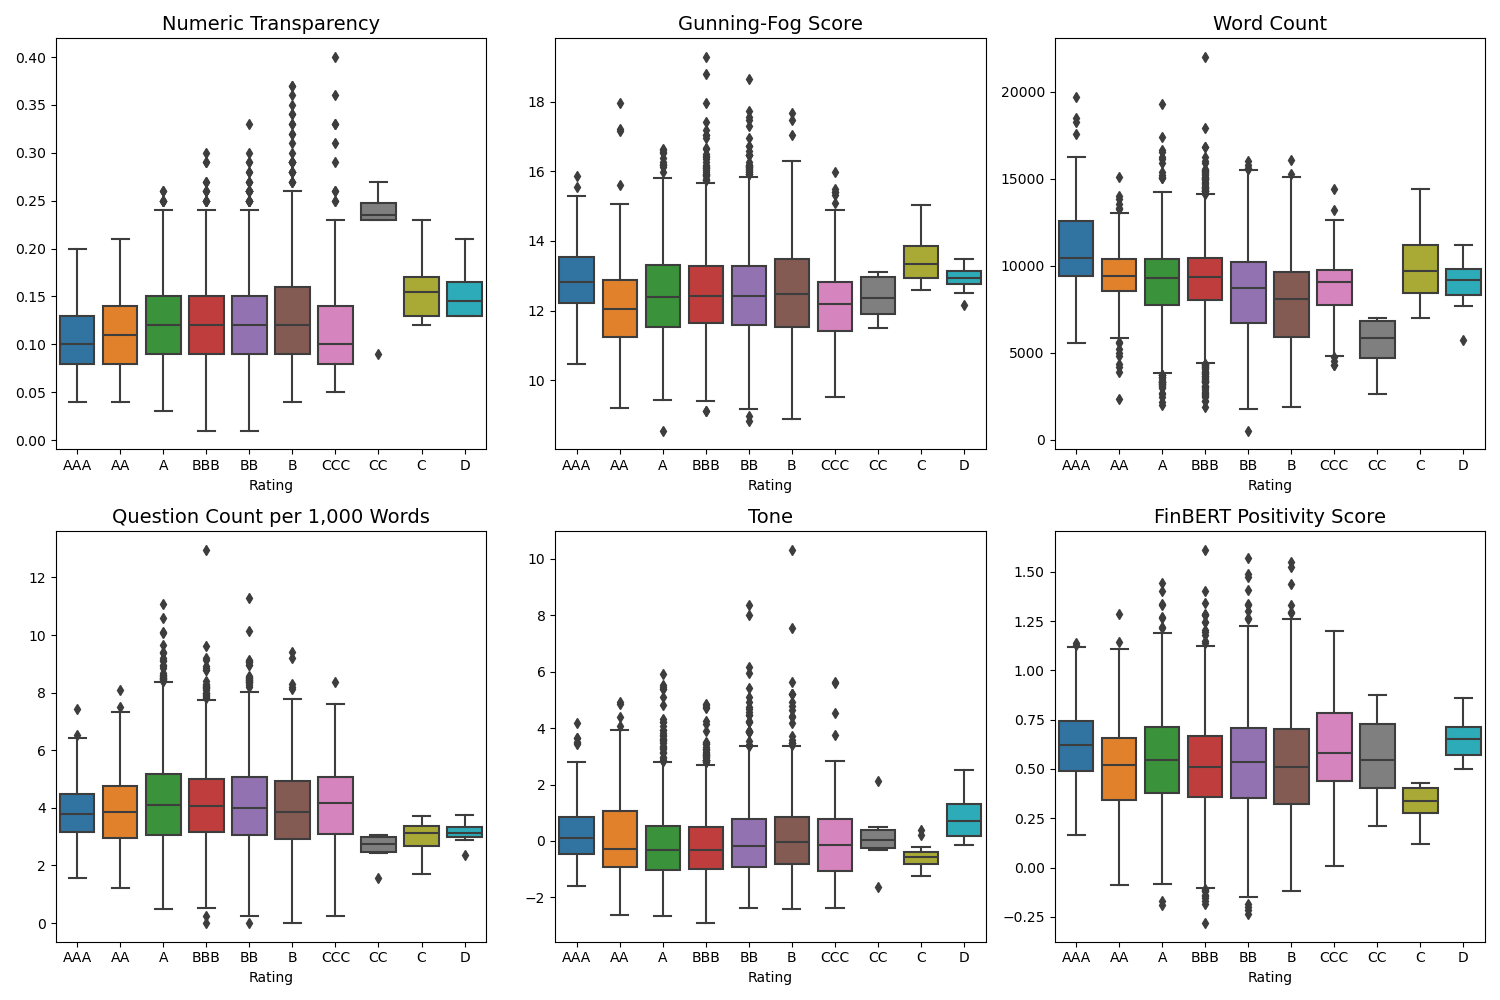
\includegraphics[width=0.6\linewidth,keepaspectratio=true]{../Output/NLP/hist_by_rating.png}
        \label{fig:dist-nlp-by-rating}
	\end{figure}

    \section*{Network of Firms}

    In addition to our standard NLP features, which already capture a rich representation, we also created a network graph representing the connections between firms based on mentions within calls. We deployed transformer-based named-entity recognition \citep{spacy_spacy_2024} to identify company names in the text, then cleaned and matched these names to standardized versions.\footnote{Interestingly, we found that simple code to remove words such as ``Company'', ``Inc.'', etc. followed by an exact match ignoring case outperformed fuzzy matching algorithms such as Levenshtein distance and q-gram similarity.} An interactive visualization of our entire network of firms (aggregating mentions up from the call level - where we also have a network) can be found at \url{https://sites.google.com/view/isaac-liu/company-mentions-network}, and a ~50\% sample of nodes (faster load time) can be found at \url{https://sites.google.com/view/isaac-liu/co-mentions-50-node-sample}.

    \section*{Modelling}

    Our overall model architecture is of the form

    \begin{equation*}
        \text{Predicted Credit Rating} = f(\text{Altman's Z}, \text{Financial Variables}, \text{Sector}, \text{NLP Features})
    \end{equation*}

    We performed an 80-20 train-test split on our data (\trainCount \space train, \testCount \space test), and used 5-fold cross validation to select hyperparameters for the Logistic Regression and XGBoost models.

    \subsection*{Logistic Regression}

    Table \ref{tab:logistic-regression-model-comparison} shows prediction statistics for our initial set of classifiers - simple and interpretable logistic regression models aiming to predict ratings. In the main section of this paper, we do not include the rating on the previous fixed quarter date (for those results, see Appendix Section \ref{sec:include-previous-rating}). For predicting changes in rating, see Appendix Section \ref{sec:change-prediction}.
    
    \begin{table*}[h!]
        \centering
        \caption{Logistic Regression Model Comparison}
        \footnotesize
\begin{tabular}{ccc}
\toprule
Model/Baseline & Accuracy & Share $\le$ 1 Rating From Actual \\
\midrule
Altman's Z & 0.1923 & 0.4633 \\
Financial Variables and Sector & 0.6225 & 0.9186 \\
Financial Variables, Sector, and NLP Features & 0.6333 & 0.9267 \\
Most Common Class Baseline & 0.3247 &  \\
\bottomrule
\end{tabular}

\normalsize
        \label{tab:logistic-regression-model-comparison}
    \end{table*}

    Altman's Z-Score alone performs poorly - worse than simply assuming each rating belonged to the most common class.\footnote{This model also does not significantly outperform a random guess model based on the distribution or ratings in the training dataset, which achieved an accuracy of \ratingRGAcc.} Substantial improvement can be attained by instead using underlying and additional financial variables (for a list, see Table \ref{tab:financial_summary_statistics}) as well as sector, and a slight further improvement by adding our NLP features - though this second improvement is not statistically significant (we made use of McNemar's test for all significance checks in this paper - see Appendix Section \ref{sec:mcnemars-test}). These models including financial variables very frequently bring the predicted rating one rating or less away from the actual.

    \begin{table*}[h!]
        \centering
        \caption{Confusion Matrix and Permutation Importance - Most Complex Logistic Regression Model}
        \begin{minipage}[c]{0.45\linewidth}
            \centering
            %\caption{\footnotesize Classification Report - Most Complex Model} 
            %\input{../Output/Modelling/Logistic Regression/exclude_previous_rating_model_3/exclude_previous_rating_model_3_confusion_matrix_no_title.png}
            %\label{tab:most-complex-classification-report}
            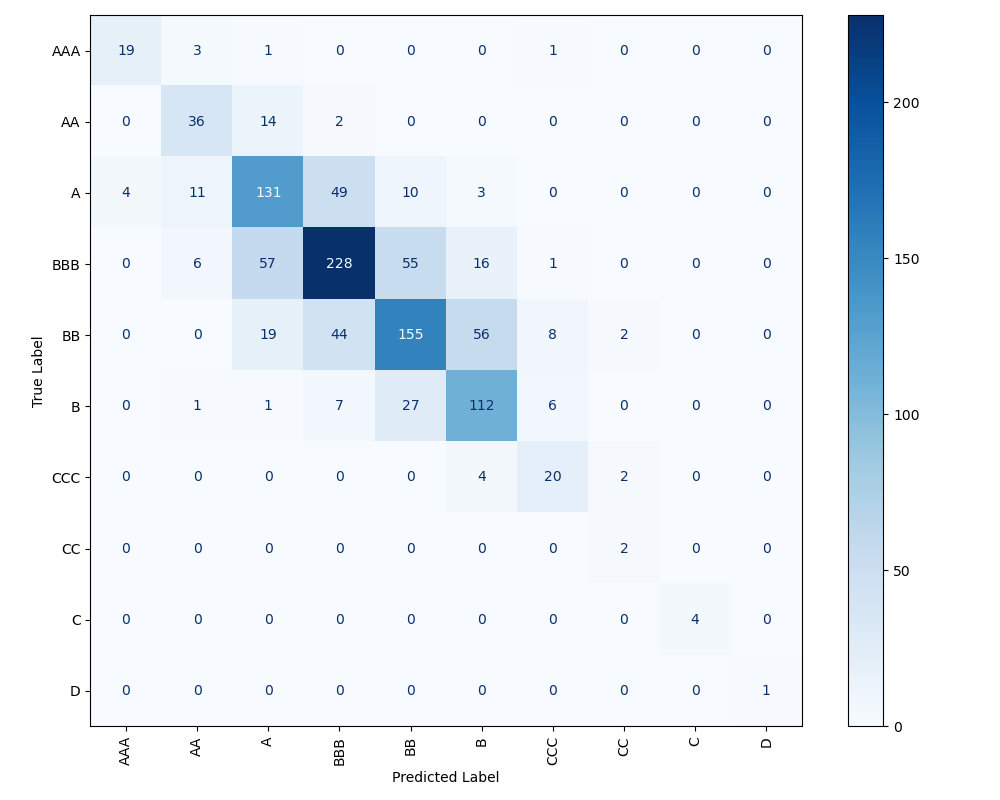
\includegraphics[width=0.95\hsize]{../Output/Modelling/Logistic Regression/exclude_previous_rating_model_3/exclude_previous_rating_model_3_confusion_matrix_no_title.png}
        \end{minipage}
        \begin{minipage}[c]{0.45\linewidth}
            \centering
            %\caption{\footnotesize Permutation Importance - Most Complex Model} 
            \tiny
\begin{tabular}{ccc}
\toprule
Permuted Feature & Mean Accuracy Drop & Standard Deviation \\
\midrule
Ratio E & 0.070625 & 0.009156 \\
Passive Tone & 0.056786 & 0.007741 \\
Sector: Utilities & 0.043208 & 0.005661 \\
Interest Expense & 0.043019 & 0.007802 \\
Ratio D & 0.041765 & 0.007607 \\
Ratio C & 0.040578 & 0.008042 \\
Depreciation and Amortization (Income Statement) & 0.038593 & 0.007163 \\
Net Receivables & 0.036435 & 0.007130 \\
Word Count & 0.035743 & 0.007747 \\
Long-Term Debt & 0.035463 & 0.007198 \\
Market Capitalization & 0.031103 & 0.006867 \\
Goodwill and Intangible Assets & 0.030084 & 0.007430 \\
Gross Profit & 0.027059 & 0.006837 \\
Total Debt & 0.026485 & 0.007413 \\
Net Debt & 0.025156 & 0.007661 \\
\bottomrule
\end{tabular}

\normalsize
            %\label{tab:most-complex-permutation-importance}
        \end{minipage}
        \label{tab:logistic-most-complex-confusion-matrix-and-permutation-importance}
    \end{table*}

    The left side of Table \ref{tab:logistic-most-complex-confusion-matrix-and-permutation-importance} shows that our most complex model with financial and NLP features generally performs well across all classes (for details, see Appendix Section \ref{sec:logistic-most-complex-model-additional-details}). This is in large part due to our use of balanced class weighting to handle rare classes. We also found via grid search that an Elastic Net penalty (which collapses to entirely a LASSO penalty) with a slight amount of regularization (C) effectively handles the large number of variables present in our data. The right side of Table \ref{tab:logistic-most-complex-confusion-matrix-and-permutation-importance} shows the 15 most important individual features as determined by the average drop in test accuracy when the feature is permuted 1,000 times. Financial features appear to be the most important, with some contributions from our NLP features considering tone and word count.

    \subsection*{XGBoost}

    In Table \ref{tab:xgboost-model-comparison}, we used the popular gradient boosting algorithm XGBoost to predict ratings, finding significant success. With the ability to model complex interactions between variables, we are able to attain substantially higher accuracy when including financial variables, and NLP features provide a statistically significant additional benefit. At around 90\% accuracy, our best model attains a level of performance slightly exceeding that in \cite{das_credit_2023}, with the substantially harder prediction task of predicting from among 10 different ratings (rather than a binary investment grade versus junk classification), and without the affordances of a graph neural network or more complex ensembling. Our model is near perfect in placing ratings within a very close neighborhood of their actual values.

    \begin{table*}[h!]
        \centering
        \caption{XGBoost Model Comparison}
        \footnotesize
\begin{tabular}{ccc}
\toprule
Model/Baseline & Accuracy & Share $\le$ 1 Rating From Actual \\
\midrule
Altman's Z & 0.3855 & 0.7657 \\
Financial Variables and Sector & 0.7630 & 0.9597 \\
Financial Variables, Sector, and NLP Features & 0.9034 & 0.9857 \\
Most Common Class Baseline & 0.3247 &  \\
\bottomrule
\end{tabular}

\normalsize
        \label{tab:xgboost-model-comparison}
    \end{table*}

    Table \ref{tab:xgboost-most-complex-confusion-matrix-and-permutation-importance} demonstrates that this strong performance by our most complex model is consistent across all classes. Our selected hyperparameters, described in detail in Appendix Section \ref{sec:xgboost-most-complex-model-additional-details}, appear to have worked well on this dataset. Financial features appear to be the most important individual variables, though NLP features also contribute in aggregate (FinBERT positivity, the negative and understated components of tone, and numeric transparency contribute substantially at rank \rPosScoreFinbert, \rNeg, and \rUndrst \space respectively - word count less so, at rank \rWordCount).\footnote{Given that our specific tone components are counts of words, they may have absorbed some of the predictive power of the word count feature in this case.} Relative to prior work, our addition of far more financial factors, in combination with complex and transformer-based NLP features, in our large dataset, appears to greatly improve performance.

    \begin{table*}[h!]
        \centering
        \caption{Confusion Matrix and Permutation Importance - Most Complex XGBoost Model}
        \begin{minipage}[c]{0.45\linewidth}
            \centering
            %\caption{\footnotesize Classification Report - Most Complex Model} 
            %\footnotesize
\begin{tabular}{ccccc}
\toprule
Rating & Precision & Recall & F1-Score & Support \\
\midrule
A & 0.8447 & 0.8894 & 0.8665 & 208 \\
AA & 0.8824 & 0.5769 & 0.6977 & 52 \\
AAA & 0.9048 & 0.7917 & 0.8444 & 24 \\
B & 0.9272 & 0.9091 & 0.9180 & 154 \\
BB & 0.9357 & 0.9225 & 0.9291 & 284 \\
BBB & 0.9129 & 0.9532 & 0.9326 & 363 \\
C & 1.0000 & 1.0000 & 1.0000 & 4 \\
CC & 1.0000 & 0.5000 & 0.6667 & 2 \\
CCC & 0.7857 & 0.8462 & 0.8148 & 26 \\
D & 1.0000 & 1.0000 & 1.0000 & 1 \\
\bottomrule
\end{tabular}

\normalsize
            %\label{tab:most-complex-classification-report}
            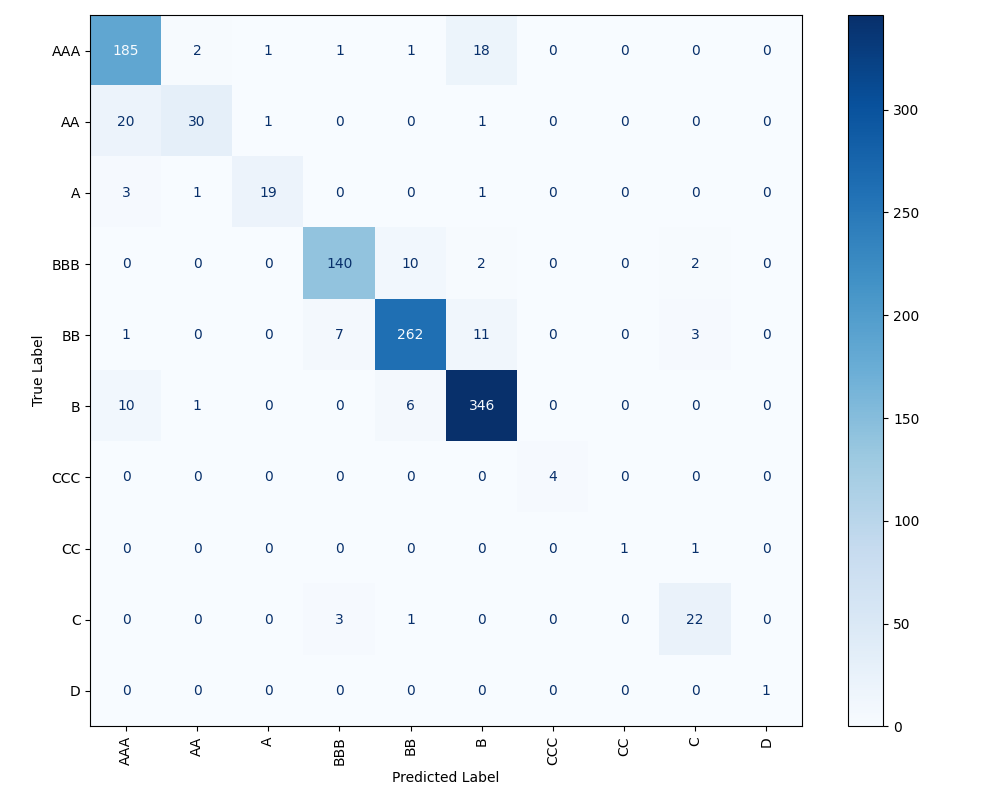
\includegraphics[width=0.95\hsize]{../Output/Modelling/XGBoost/exclude_previous_rating_model_3/exclude_previous_rating_model_3_confusion_matrix_no_title.png}
        \end{minipage}
        \begin{minipage}[c]{0.45\linewidth}
            \centering
            %\caption{\footnotesize Permutation Importance - Most Complex Model} 
            \tiny
\begin{tabular}{ccc}
\toprule
Permuted Feature & Mean Accuracy Drop & Standard Deviation \\
\midrule
Retained Earnings & 0.043819 & 0.005761 \\
Market Capitalization & 0.035169 & 0.005735 \\
Dividends Paid & 0.021455 & 0.004481 \\
Debt Ratio & 0.009987 & 0.003413 \\
Common Stock & 0.009693 & 0.002248 \\
Ratio E & 0.009535 & 0.003463 \\
Other Total Stockholders' Equity & 0.009288 & 0.003028 \\
Total Current Liabilities & 0.006888 & 0.002785 \\
Inventory (Balance Sheet) & 0.006802 & 0.002994 \\
Total Current Assets & 0.006684 & 0.003243 \\
Selling General and Administrative Expenses & 0.006031 & 0.002395 \\
Interest Expense & 0.005973 & 0.002740 \\
Net Property Plant Equipment & 0.005729 & 0.001915 \\
Ratio C & 0.005677 & 0.002476 \\
Total Non-Current Assets & 0.005589 & 0.003420 \\
\bottomrule
\end{tabular}

\normalsize
            %\label{tab:most-complex-permutation-importance}
        \end{minipage}
        \label{tab:xgboost-most-complex-confusion-matrix-and-permutation-importance}
    \end{table*}

    \subsection*{Graph Neural Network}

    We make use of the network of company mentions within earnings calls to train an end-to-end graph neural network for classification. Graph Neural Networks construct powerful representations of nodes/entities in a network of relationships by using message passing to aggregate features from neighboring nodes. In this work, we use a GraphSAGE \citep{hamilton_inductive_2018} Graph Convolutional Network (GCN) implemented via the Deep Graph Library. For details concerning our network architecture, see Appendix Section \ref{sec:gnn-architecture}.

    % end lyx insertion

    To initialize our network, we form an unweighted and undirected edge connection between nodes of firm by fixed quarters based on the full firm to firm graph (which was aggregated across quarters) discussed earlier. Our network consists of subgraphs for each fixed quarter date. If two firms are ever connected via a mention, their nodes are always connected within each fixed quarter date. When we include only nodes that are connected to others, and nodes for rating classes with more than one value in the training data, we are left with \numNodes \space nodes (\numTrainNodes \space training, \numTestNodes \space test) falling into \gnnNumClasses \space rating classes, and \numEdges \space edges between these company-quarters. The average degree of the network is \averageDegree \space connections.

    For reference, we also constructed comparisons with our other classifiers including financial and NLP features on the graph neural network's dataset. Logistic regression and XGBoost achieved an accuracies of \pretrainedLRAccuracy \space and \pretrainedXGBAccuracy \space on the graph neural network's test set. A possibly fairer comparison are the accuracies we achieved on this set after fully retraining these classifiers (albeit with the same hyperparameters as earlier) on the graph neural network's training set, which were \retrainLRAccuracy \space and \retrainXGBAccuracy.

    \begin{table*}[h!]
        \centering
        \caption{Transductive Graph Neural Network Model Comparison and Confusion Matrix for Most Complex Model}
        \begin{minipage}[c]{0.495\linewidth}
            \centering
            \footnotesize
\begin{tabular}{cc}
\toprule
Model/Baseline & Accuracy \\
\midrule
Altman's Z & 0.3134 \\
Financial Variables and Sector & 0.5249 \\
Financial Variables, Sector, and NLP Features & 0.4925 \\
Most Common Class Baseline & 0.2985 \\
\bottomrule
\end{tabular}

\normalsize
        \end{minipage}
        \begin{minipage}[c]{0.495\linewidth}
            \centering
            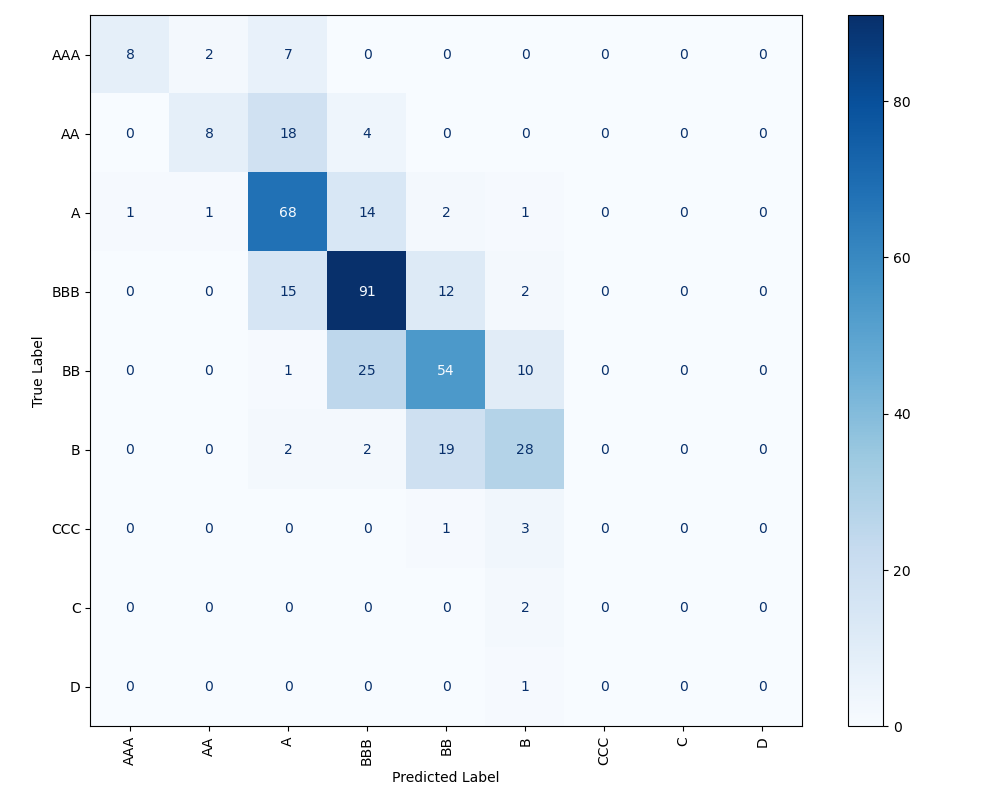
\includegraphics[width=0.95\hsize]{../Output/Modelling/Graph Neural Network/Transductive/confusion_matrix_no_title.png}
        \end{minipage}
        \label{tab:transductive-model-comparison-and-confusion-matrix}
    \end{table*}

    Graph Neural Networks for node classification may be trained transductively or inductively. In the transductive setting, the entire graph of firms - the training and test dataset, and their associated features - is visible to the model for training, but the labels for the test dataset are masked. Therefore, the model is retrained when a new node for which a prediction is to be made is added. The performance for our transductive models is shown in Table \ref{tab:transductive-model-comparison-and-confusion-matrix}. Our performance is slightly better than that of logistic regression (statistically significant relative to the retrained, though not pretrained version) but trails that of XGBoost,\footnote{It is sometimes stated that XGBoost and tree-based algorithms can outperform neural networks on heterogenous data - our diverse collection of variables from a variety of sources fall in line with such an explanation.} and similar to the logistic case, NLP features do not clearly contribute.

    \begin{table*}[h!]
        \centering
        \caption{Inductive Graph Neural Network Model Comparison and Confusion Matrix for Most Complex Model}
        \begin{minipage}[c]{0.495\linewidth}
            \centering
            \footnotesize
\begin{tabular}{cc}
\toprule
Model/Baseline & Accuracy \\
\midrule
Altman's Z & 0.3092 \\
Financial Variables and Sector & 0.6234 \\
Financial Variables, Sector, and NLP Features & 0.6085 \\
Most Common Class Baseline & 0.2993 \\
\bottomrule
\end{tabular}

\normalsize
        \end{minipage}
        \begin{minipage}[c]{0.495\linewidth}
            \centering
            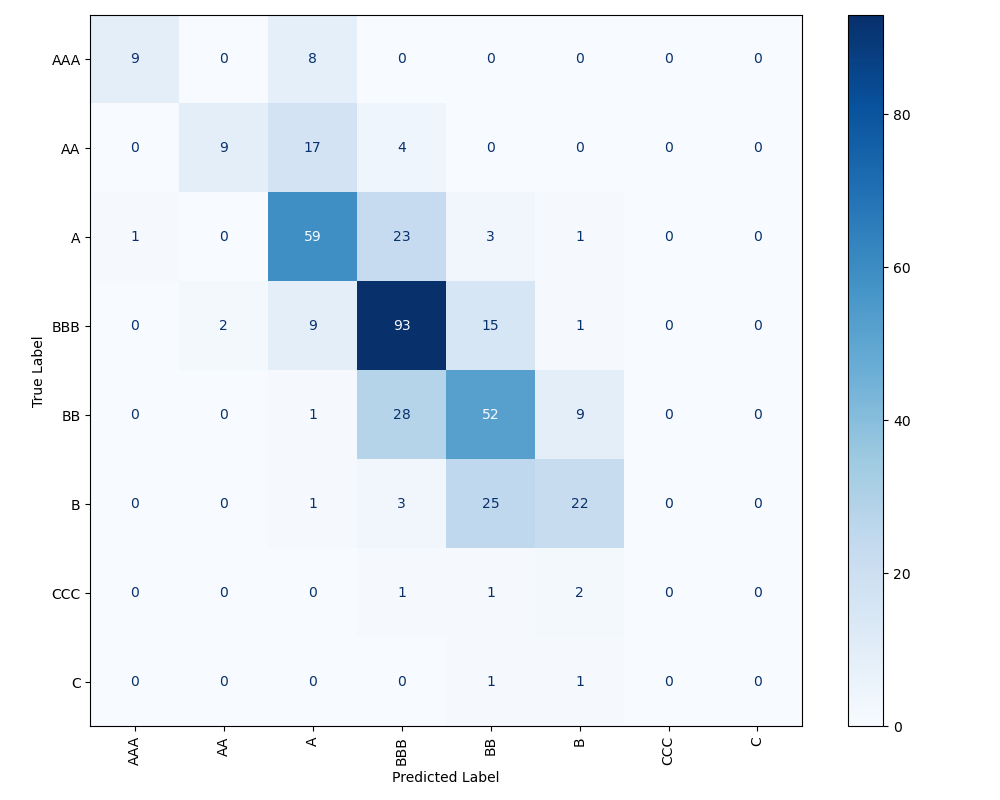
\includegraphics[width=0.95\hsize]{../Output/Modelling/Graph Neural Network/Inductive/confusion_matrix_no_title.png}
        \end{minipage}
        \label{tab:inductive-model-comparison-and-confusion-matrix}
    \end{table*}


    In the inductive setting, introduced in \cite{hamilton_inductive_2018} with GraphSAGE, the model can only see the network of nodes in the training dataset, and uses this to learn general functions for embedding nodes. This makes the model easier to adapt to new data, but may come at some cost to performance. Our inductive results are shown in Table \ref{tab:inductive-model-comparison-and-confusion-matrix}, and are similar to (and not significantly different from) the transductive case, though differences with both logistic regression models are now significant.

    \section*{Conclusion}

    In this paper we demonstrated methods to incorporate the text of earnings call transcripts to improve predictions of corporate credit ratings. Simple logistic regression achieves middling accuracy on the difficult task of rating prediction, which is not signficantly improved by the addition of NLP features. When we implement XGBoost to better account for interactions between variables, however, performance reaches state-of-the-art/near-state-of-the-art levels, with a substantial contribution from NLP features. Our experimental graph neural network based on mentions of other companies calls behaved somewhat in-between these two methods. We have a moderate degree of evidence that NLP features are important within our specific setup when used with a sufficiently capable classifier, and most of them (particularly aspects of tone, positivity, numeric transparency, and word count) contribute in at least some models.

    There remains substantial opportunity for future improvements to this project. We would have liked to incorporate more metadata for our calls and financial information into predictions, leveraging date and time series components. Though our XGBoost classifier already performs well, with more time we would have liked to explore more hyperparameters to further improve accuracy.\footnote{We based our initial hyperparameter settings and grid in part on optimal results from the Autogluon AutoML library \citep{erickson_autogluon_2024} for a model similar to our most complex one, but we would have loved to explore more starting points for our exact final model also using Bayesian optimization (potentially from other libraries).} We experimented with the use of Doc2Vec embedding cosine similarities for network construction on our data (which seemed to work well in \cite{das_credit_2023}), but instead opted to use more interpretable mentions to train our classifier. A different foundational approach would be to extract node embeddings from our graph neural network and use them with another classifier (likely XGBoost). We also might make specific adjustments to our architecture to handle individual fixed quarter date subgraphs, and incorporate weighted edges for the number of actual mentions.\footnote{We might also consider forming connections between nodes for the same company across time, though such a modification may also introduce undesired heterogeneity in the meaning of an edge.} Overall, it seems likely that mastery of credit rating prediction, especially when including rich representations of text from earnings calls, is within reach of machine learning models.

    \section*{Acknowledgements}

    Special thanks to the UC Berkeley Stats Department Statistical Computing Facility (SCF). Other acknowledgements: Libor Pospisil, Robert Thompson. GitHub Co-Pilot was used for python code generation (mostly for plotting and table creation/parsing).

    \clearpage
    \newpage

    \bibliographystyle{aea}
    \bibliography{Stat-222-Capstone}

    \clearpage
    \newpage

    \appendix

    % Reset and change numbering for figures and tables
    \counterwithin{figure}{section}
    \counterwithin{table}{section}

    \section{Appendix}

    \subsection{Example of One Observation in Final Data}

    \label{sec:one-obs-final-data}

    Figure \ref{fig:one-obs-final-data} shows some variables for Apple Inc. for the fixed quarter date of October 1, 2014. Apple had a strong rating of AA at this time. This was supported, in part, by a relatively high Altman Z-Score, capturing the company's excellent financial condition. Sentiment and tone of the earnings call for this quarter were generally positive, numeric transparency indicates there was a relatively high share of words to numbers (indicating more potentially bold commentary), and word count/call length was around average.

    \begin{figure*}[h]
        \caption{Apple Inc., October 1, 2014}
        \begin{subfigure}[h]{0.4925\textwidth}
            \centering
            \subcaption*{Metadata, Rating, and NLP Features}
            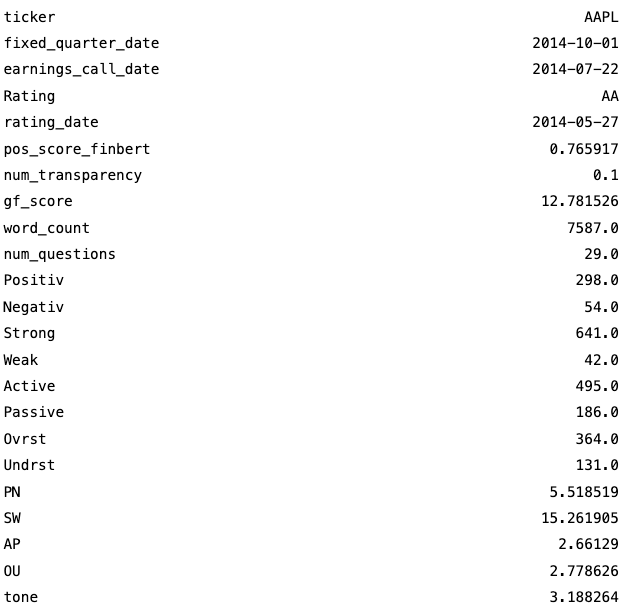
\includegraphics[width=0.95\hsize]{../Output/NLP/aapl nlp.png}
        \end{subfigure}
        %\hfill
        \begin{subfigure}[h]{0.4925\textwidth}
            \centering
            \subcaption*{Financial Data}
            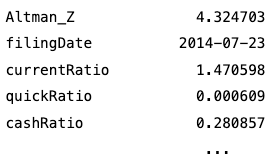
\includegraphics[width=0.5\hsize]{../Output/NLP/aapl fin.png}
        \end{subfigure}
        \hfill
        \label{fig:one-obs-final-data}
    \end{figure*}

    \clearpage
    \newpage

    \subsection{Observations by Quarter and Year}

    Figure \ref{fig:obs-by-quarter-year} demonstrates that the data is temporally unbalanced, with many companies entering the dataset in later years, after they first receive an observable credit rating.

    \begin{figure}[h!]
		\centering
        \caption{Observations by Quarter and Year}
        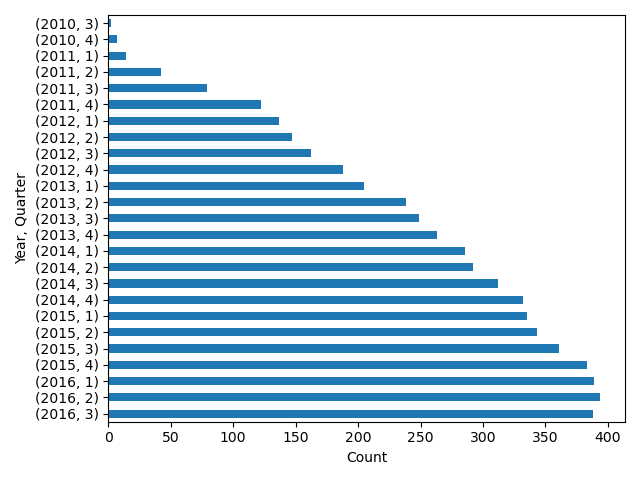
\includegraphics[width=0.6\linewidth,keepaspectratio=true]{../Output/All Data EDA/Tabular EDA/all_data_fixed_quarter_dates_obs_by_year_quarter_no_title.png}
        \label{fig:obs-by-quarter-year}
	\end{figure}

    \clearpage
    \newpage

    \subsection{Data Cleaning Steps}

    \label{sec:data-cleaning}

    To ensure comparability, we dropped items missing any predictor variable, as well as some companies with only a few (3 or less) quarters. 
    
    We identified one bankruptcy in our data - Peabody Energy on April 13, 2016 - and on further investigation, deleted some quarters with incorrect ratings. 
    
    We removed all calls that happened more than 250 days prior and after the first day of the year and quarter they are supposed to discuss the results from, as well as calls for companies that hold them on an annual, rather than quarterly basis.

    For our financial data, we limited our observations to items reported in USD, checked for and corrected values off by a factor of 1,000 as a result of parsing,\footnote{If the last few digits were 000.00 and the item was above or below the 2.5\% and 97.5\% quantile, we divided by 1,000.} and checked some accounting identities in \cite{das_credit_2023},\footnote{We checked total liabilities were greater than current liabilities, total assets were greater than total current assets, and net sales (revenue) was greater than EBIT. We originally also checked that total assets were greater than or equal to total equity + retained earnings + total liabilities, but this proved to be too restrictive.} setting failing variables to missing. We also discarded observations where statement filing dates did not agree between the three types of statements (income statement, balance sheet, and cash flow statement), where the filing date fell outside of the fixed quarter matched on via earnings call date, and where the filing date was more than 45 days after the earnings call date.

    We removed observations with outliers for any NLP feature, produced, for example, as a result of zeroes or low values in denominators.

    \clearpage
    \newpage

    \subsection{Summary Statistics for Financial Variables}

    \label{sec:financial-summary-statistics}

    Table \ref{tab:financial_summary_statistics} shows summary statistics for the financial variables we include in our models (including sub-components of Altman's Z Score) in our final prepared data.\footnote{We did not Winsorize all of our financial ratios (though we could have) due to general agreement on even extreme values with \cite{das_credit_2023}.} Other important variables are explained in the main text.

    \tiny
\begin{longtable}{ccccccc}
\caption{Financial Variable Summary Statistics} \label{tab:financial_summary_statistics} \\
\toprule
Variable Name & Mean & Minimum & Median & Maximum & Standard Deviation & Variable Type \\
\midrule
\endfirsthead
\caption[]{Financial Variable Summary Statistics} \\
\toprule
Variable Name & Mean & Minimum & Median & Maximum & Standard Deviation & Variable Type \\
\midrule
\endhead
\midrule
\multicolumn{7}{r}{Continued on next page} \\
\midrule
\endfoot
\bottomrule
\endlastfoot
Cash Per Share & 4.57 & 0.00 & 2.13 & 69.91 & 9.64 & Additional Ratios \\
Cash Ratio & 1.21 & 0.00 & 0.28 & 53.17 & 6.23 & Additional Ratios \\
Current Ratio & 1.93 & 0.35 & 1.58 & 7.93 & 1.33 & Additional Ratios \\
Debt Ratio & 0.35 & 0.00 & 0.32 & 0.94 & 0.19 & Additional Ratios \\
Debt Ratio (Alternative Definition) & 0.65 & 0.28 & 0.64 & 1.22 & 0.17 & Additional Ratios \\
Debt to Equity Ratio & -34.63 & -1,890.41 & 1.70 & 25.40 & 256.02 & Additional Ratios \\
EBIT to Revenue & 0.12 & -0.26 & 0.11 & 0.47 & 0.12 & Additional Ratios \\
Enterprise Value Multiplier & 59.08 & -309.75 & 40.67 & 727.20 & 125.93 & Additional Ratios \\
Equity Multiplier & -22.79 & -1,270.10 & 2.71 & 22.64 & 175.08 & Additional Ratios \\
Free Cash Flow Per Share & 0.57 & -2.98 & 0.39 & 7.70 & 1.52 & Additional Ratios \\
Free Cash Flow to Operating Cash Flow & 0.72 & -2.42 & 0.66 & 10.98 & 1.86 & Additional Ratios \\
Operating Cash Flow Per Share & 1.48 & -0.98 & 1.04 & 11.82 & 1.92 & Additional Ratios \\
Operating Cash Flow to Sales & 0.16 & -0.15 & 0.14 & 0.64 & 0.15 & Additional Ratios \\
Quick Ratio & 1.36 & 0.00 & 1.15 & 6.12 & 0.98 & Additional Ratios \\
Return on Assets & 0.01 & -0.03 & 0.01 & 0.06 & 0.02 & Additional Ratios \\
Return on Capital Employed & 0.03 & -0.03 & 0.02 & 0.11 & 0.03 & Additional Ratios \\
Return on Equity & 0.01 & -1.32 & 0.03 & 0.78 & 0.25 & Additional Ratios \\
Accounts Payable (Balance Sheet) & 957,290,323.93 & -237,651,171.00 & 356,700,000.00 & 11,433,000,000.00 & 1,551,108,353.02 & Financial Statements \\
Accounts Payable (Cash Flow Statement) & 5,154,565.15 & -321,769,000.00 & 0.00 & 1,789,652,000.00 & 82,110,968.91 & Financial Statements \\
Accounts Receivables & -11,478,236.25 & -544,000,000.00 & 0.00 & 325,000,000.00 & 91,535,961.30 & Financial Statements \\
Accumulated Other Comprehensive Income (Loss) & -404,483,300.22 & -5,290,000,000.00 & -77,514,000.00 & 431,595,000.00 & 874,353,108.41 & Financial Statements \\
Capital Expenditure & -192,514,484.47 & -1,867,000,000.00 & -60,129,000.00 & 412,700.00 & 310,057,440.27 & Financial Statements \\
Capital Lease Obligations & 24,642,498.79 & 0.00 & 0.00 & 9,056,234,000.00 & 228,328,885.18 & Financial Statements \\
Cash and Cash Equivalents & 862,135,865.07 & 0.00 & 333,000,000.00 & 9,223,000,000.00 & 1,366,595,243.17 & Financial Statements \\
Cash and Short Term Investments & 1,060,086,810.64 & 0.00 & 363,008,000.00 & 15,601,000,000.00 & 1,890,682,420.93 & Financial Statements \\
Cash at Beginning of Period & 867,410,489.82 & -2,556,000.00 & 334,000,000.00 & 9,610,000,000.00 & 1,388,834,800.13 & Financial Statements \\
Cash at End of Period & 871,017,693.39 & -154,400.00 & 335,469,000.00 & 9,743,000,000.00 & 1,394,641,397.30 & Financial Statements \\
Change in Working Capital & -17,557,103.20 & -870,000,000.00 & -2,384,000.00 & 753,000,000.00 & 183,788,257.05 & Financial Statements \\
Common Stock & 329,277,684.36 & -539,800.00 & 3,800,000.00 & 9,817,134,000.00 & 925,626,949.20 & Financial Statements \\
Common Stock Issued & 44,672,509.36 & -3,572,000.00 & 43,000.00 & 1,111,490,728.00 & 124,027,450.20 & Financial Statements \\
Common Stock Repurchased & -78,527,033.90 & -2,086,545,366.00 & -773,000.00 & 545,656,614.52 & 188,219,352.34 & Financial Statements \\
Cost and Expenses & 2,317,513,877.07 & -2,495,000.00 & 1,121,064,000.00 & 22,769,000,000.00 & 3,357,899,606.58 & Financial Statements \\
Cost of Revenue & 1,624,233,369.18 & -3,094,000.00 & 787,700,000.00 & 18,303,000,000.00 & 2,405,765,370.43 & Financial Statements \\
Debt Repayment & -247,880,234.24 & -3,001,000,000.00 & -33,400,000.00 & 200.00 & 471,724,050.37 & Financial Statements \\
Deferred Income Tax & 6,154,669.54 & -253,000,000.00 & 64,000.00 & 1,850,454,000.00 & 58,927,713.28 & Financial Statements \\
Deferred Revenue & 310,000,739.66 & -116,912,000.00 & 50,066,000.00 & 4,918,100,000.00 & 642,489,899.31 & Financial Statements \\
Depreciation and Amortization (Cash Flow Statement) & 141,811,048.14 & -675,312.00 & 53,551,000.00 & 1,529,000,000.00 & 210,315,836.18 & Financial Statements \\
Depreciation and Amortization (Income Statement) & 140,571,212.83 & -1,550,000.00 & 54,507,000.00 & 1,371,000,000.00 & 203,167,331.44 & Financial Statements \\
Diluted EPS & 0.51 & -156.36 & 0.51 & 49.73 & 3.31 & Financial Statements \\
Dividends Paid & -91,357,096.76 & -1,233,000,000.00 & -21,054,000.00 & 0.00 & 182,429,714.55 & Financial Statements \\
EBITDA & 444,995,396.82 & -66,200,000.00 & 193,000,000.00 & 4,410,000,000.00 & 644,706,471.62 & Financial Statements \\
EBITDA Ratio & 0.20 & -5.77 & 0.17 & 2.16 & 0.22 & Financial Statements \\
EPS & 0.52 & -156.36 & 0.52 & 53.75 & 3.33 & Financial Statements \\
Effect of Foreign Exchange Changes on Cash & -1,697,085.83 & -65,000,000.00 & 0.00 & 52,000,000.00 & 11,200,007.88 & Financial Statements \\
Free Cash Flow & 156,892,657.81 & -541,000,000.00 & 51,691,000.00 & 2,683,000,000.00 & 389,666,937.19 & Financial Statements \\
General and Administrative Expenses & 153,933,016.99 & -2,738,500.00 & 33,768,000.00 & 2,007,000,000.00 & 303,900,948.38 & Financial Statements \\
Goodwill & 2,009,260,205.06 & -202,702,100.00 & 636,039,000.00 & 23,389,000,000.00 & 3,554,057,246.39 & Financial Statements \\
Goodwill and Intangible Assets & 3,102,882,804.88 & -1,618,944,000.00 & 970,000,000.00 & 37,123,000,000.00 & 5,639,038,312.52 & Financial Statements \\
Gross Profit & 861,821,178.07 & -7,195,000.00 & 378,500,000.00 & 9,223,000,000.00 & 1,365,410,717.45 & Financial Statements \\
Gross Profit Ratio & 0.37 & -5.65 & 0.34 & 2.32 & 0.26 & Financial Statements \\
Income Before Tax & 255,351,974.53 & -353,153,000.00 & 91,900,000.00 & 2,951,000,000.00 & 434,623,029.43 & Financial Statements \\
Income Before Tax Ratio & 0.07 & -9.38 & 0.09 & 2.68 & 0.35 & Financial Statements \\
Income Tax Expense & 69,444,774.33 & -119,131,000.00 & 22,100,000.00 & 736,000,000.00 & 121,681,731.43 & Financial Statements \\
Intangible Assets & 835,940,509.51 & -421,000.00 & 170,197,000.00 & 14,110,100,000.00 & 1,785,542,119.17 & Financial Statements \\
Interest Expense & 46,568,508.69 & -16,400,000.00 & 23,000,000.00 & 386,000,000.00 & 61,712,161.15 & Financial Statements \\
Interest Income & 2,372,725.23 & -62,900.00 & 0.00 & 69,000,000.00 & 6,859,086.75 & Financial Statements \\
Inventory (Balance Sheet) & 933,043,177.40 & -19,626,000.00 & 403,789,000.00 & 8,328,000,000.00 & 1,398,934,358.21 & Financial Statements \\
Inventory (Cash Flow Statement) & -10,302,495.14 & -420,000,000.00 & 0.00 & 289,000,000.00 & 70,374,129.32 & Financial Statements \\
Investments in Property, Plants, and Equipment & -193,897,744.95 & -1,921,864,000.00 & -60,373,000.00 & 412,700.00 & 313,436,441.14 & Financial Statements \\
Long-Term Debt & 4,159,473,460.27 & -651,718.00 & 1,822,139,000.00 & 31,359,000,000.00 & 5,574,538,232.32 & Financial Statements \\
Long-Term Investments & 494,196,440.41 & -490,677,000.00 & 12,449,000.00 & 10,981,000,000.00 & 1,359,571,399.50 & Financial Statements \\
Minority Interest & 90,043,651.07 & -20,252,654.04 & 1,600,000.00 & 2,316,406,000.00 & 268,200,905.93 & Financial Statements \\
Net Acquisitions & -32,878,764.18 & -805,960,000.00 & 0.00 & 249,000,000.00 & 116,107,004.20 & Financial Statements \\
Net Cash Provided by Operating Activities & 352,446,106.81 & -179,404,000.00 & 143,626,000.00 & 3,870,000,000.00 & 545,602,564.63 & Financial Statements \\
Net Cash Used for Investing Activities & -252,575,304.44 & -2,840,033,000.00 & -71,100,000.00 & 325,900,000.00 & 443,647,871.52 & Financial Statements \\
Net Cash Used or Provided by Financing Activities & -114,570,062.00 & -2,444,000,000.00 & -29,157,000.00 & 1,094,000,000.00 & 399,330,481.52 & Financial Statements \\
Net Change in Cash & 3,933,018.18 & -1,161,000,000.00 & 573,000.00 & 1,401,000,000.00 & 269,005,283.68 & Financial Statements \\
Net Debt & 3,597,141,664.59 & -1,044,500,000.00 & 1,508,594,000.00 & 30,761,000,000.00 & 5,338,457,121.62 & Financial Statements \\
Net Income (Cash Flow Statement) & 189,122,176.12 & -327,000,000.00 & 66,190,000.00 & 2,402,000,000.00 & 336,635,167.35 & Financial Statements \\
Net Income (Income Statement) & 185,944,828.27 & -329,864,000.00 & 66,389,000.00 & 2,340,000,000.00 & 330,952,161.49 & Financial Statements \\
Net Income Ratio & 0.05 & -8.88 & 0.07 & 2.72 & 0.29 & Financial Statements \\
Net Property Plant Equipment & 4,931,687,321.78 & 0.00 & 1,389,600,000.00 & 44,441,000,000.00 & 7,885,938,319.99 & Financial Statements \\
Net Receivables & 1,276,905,848.63 & -4,199,600.00 & 570,338,000.00 & 12,116,000,000.00 & 1,776,578,353.43 & Financial Statements \\
Non-Current Deferred Revenue & 248,840,448.23 & -500,933,000.00 & 0.00 & 5,778,000,000.00 & 723,186,467.01 & Financial Statements \\
Non-Current Deferred Tax Liabilities & 702,874,797.74 & -3,818,507.00 & 135,597,000.00 & 8,306,000,000.00 & 1,400,029,509.57 & Financial Statements \\
Operating Cash Flow & 352,446,106.81 & -179,404,000.00 & 143,626,000.00 & 3,870,000,000.00 & 545,602,564.63 & Financial Statements \\
Operating Expenses & 538,189,512.49 & -13,530,000.00 & 221,700,000.00 & 6,252,000,000.00 & 918,426,909.60 & Financial Statements \\
Operating Income & 302,231,079.76 & -208,377,000.00 & 122,000,000.00 & 3,294,000,000.00 & 475,077,278.15 & Financial Statements \\
Operating Income Ratio & 0.11 & -9.71 & 0.12 & 2.86 & 0.31 & Financial Statements \\
Other Assets & 5,662.39 & -19,834,700.00 & 0.00 & 8,948,000.00 & 421,776.93 & Financial Statements \\
Other Current Assets & 370,526,390.88 & -98,000.00 & 119,600,000.00 & 4,968,950,000.00 & 664,643,317.21 & Financial Statements \\
Other Current Liabilities & 955,075,890.93 & -48,317,000.00 & 322,800,000.00 & 12,137,000,000.00 & 1,782,231,297.37 & Financial Statements \\
Other Expenses & 50,749,806.82 & -64,000,000.00 & 585,000.00 & 16,189,674,590.00 & 342,110,629.66 & Financial Statements \\
Other Financing Activities & 217,421,866.42 & -975,168,999.00 & 8,000,000.00 & 3,297,501,000.00 & 515,334,960.45 & Financial Statements \\
Other Investing Activities & 4,573,739.09 & -448,000,000.00 & 106,000.00 & 3,060,433,659.00 & 96,736,267.62 & Financial Statements \\
Other Liabilities & 95,902.58 & -3,063,000.00 & 0.00 & 51,076,000.00 & 1,967,227.53 & Financial Statements \\
Other Non-Cash Items & 15,325,139.75 & -1,848,719,007.00 & 1,621,000.00 & 703,000,000.00 & 109,294,805.79 & Financial Statements \\
Other Non-Current Assets & 506,778,121.04 & -75,012,534,818.00 & 158,696,000.00 & 8,037,000,000.00 & 1,778,143,597.09 & Financial Statements \\
Other Non-Current Liabilities & 975,892,048.39 & -286,041,895.00 & 327,700,000.00 & 11,890,564,000.00 & 1,686,827,873.95 & Financial Statements \\
Other Total Stockholders' Equity & 1,135,331,510.72 & -12,393,000,000.00 & 427,000,000.00 & 34,030,400,000.00 & 3,586,435,863.55 & Financial Statements \\
Other Working Capital & 21,414,823.22 & -1,788,851,160.00 & 0.00 & 40,341,689,407.00 & 786,599,061.35 & Financial Statements \\
Preferred Stock & 9,475,146.22 & 0.00 & 0.00 & 401,500,000.00 & 42,785,110.93 & Financial Statements \\
Purchases of Investments & -104,151,034.82 & -11,997,654,000.00 & 0.00 & 81,823,000.00 & 346,711,949.30 & Financial Statements \\
Research and Development Expenses & 28,169,938.85 & -214,000.00 & 0.00 & 893,000,000.00 & 94,071,513.75 & Financial Statements \\
Retained Earnings & 3,628,393,969.72 & -4,839,000,000.00 & 1,293,100,000.00 & 37,899,000,000.00 & 6,424,744,717.89 & Financial Statements \\
Revenue & 2,728,749,857.76 & -4,273,000.00 & 1,297,700,000.00 & 25,420,000,000.00 & 3,959,362,594.26 & Financial Statements \\
Sales and Maturities of Investments & 99,796,411.86 & -9,409,000.00 & 0.00 & 8,936,406,000.00 & 311,292,561.88 & Financial Statements \\
Selling General and Administrative Expenses & 296,899,615.00 & -5,054,000.00 & 119,600,000.00 & 3,343,000,000.00 & 486,131,457.73 & Financial Statements \\
Selling and Marketing Expenses & 25,431,647.83 & -3,003,000.00 & 0.00 & 876,761,000.00 & 97,367,023.08 & Financial Statements \\
Short Term Investments & 182,988,242.55 & -515,000.00 & 0.00 & 6,178,000,000.00 & 599,747,024.65 & Financial Statements \\
Short-Term Debt & 465,870,869.02 & -655,561.00 & 83,800,000.00 & 5,363,000,000.00 & 885,210,679.51 & Financial Statements \\
Stock-Based Compensation & 14,496,292.55 & -36,000,000.00 & 5,106,000.00 & 254,000,000.00 & 29,968,462.79 & Financial Statements \\
Tax Assets & 378,132,518.58 & -2,310,712,000.00 & 48,963,000.00 & 6,535,000,000.00 & 909,237,680.35 & Financial Statements \\
Tax Payable & 60,670,669.07 & -87,400.00 & 2,810,000.00 & 1,187,000,000.00 & 150,628,980.40 & Financial Statements \\
Total Assets & 15,592,495,985.55 & 123,279.00 & 7,048,475,000.00 & 131,119,000,000.00 & 21,911,032,910.64 & Financial Statements \\
Total Current Assets & 3,937,085,272.11 & 29,954.00 & 1,933,750,000.00 & 41,276,000,000.00 & 5,729,273,613.69 & Financial Statements \\
Total Current Liabilities & 2,811,976,684.34 & 24,083.00 & 1,138,200,000.00 & 29,919,000,000.00 & 4,247,045,840.39 & Financial Statements \\
Total Debt & 4,593,265,532.66 & 0.00 & 2,019,244,000.00 & 37,124,000,000.00 & 6,254,194,800.16 & Financial Statements \\
Total Equity & 4,968,502,543.29 & -501,467,000.00 & 2,095,000,000.00 & 49,975,000,000.00 & 7,272,421,518.55 & Financial Statements \\
Total Investments & 729,199,594.64 & -334,673,000.00 & 43,275,000.00 & 19,331,000,000.00 & 1,944,649,108.26 & Financial Statements \\
Total Liabilities & 9,817,545,124.72 & 79,283.00 & 4,308,693,000.00 & 87,293,000,000.00 & 13,527,062,565.42 & Financial Statements \\
Total Liabilities and Stockholders' Equity & 15,556,696,866.65 & 123,279.00 & 7,043,426,000.00 & 131,119,000,000.00 & 21,905,884,302.05 & Financial Statements \\
Total Liabilities and Total Equity & 15,556,696,866.65 & 123,279.00 & 7,043,426,000.00 & 131,119,000,000.00 & 21,905,884,302.05 & Financial Statements \\
Total Non-Current Assets & 11,011,964,229.49 & 49,861.00 & 4,119,200,000.00 & 104,263,000,000.00 & 15,994,777,583.25 & Financial Statements \\
Total Non-Current Liabilities & 6,639,451,321.63 & 53,696.00 & 2,809,300,000.00 & 54,300,000,000.00 & 9,424,654,097.47 & Financial Statements \\
Total Other Income Expenses Net & -13,134,652.92 & -503,976,000.00 & -920,000.00 & 286,000,000.00 & 72,414,124.07 & Financial Statements \\
Total Stockholders' Equity & 4,933,321,107.00 & -526,491,000.00 & 2,088,608,000.00 & 49,269,000,000.00 & 7,194,176,771.15 & Financial Statements \\
Weighted Average Shares Outstanding & 352,790,171.17 & 0.00 & 146,000,000.00 & 13,751,391,147.00 & 720,460,888.99 & Financial Statements \\
Weighted Average Shares Outstanding (Diluted) & 316,630,108.94 & 0.00 & 145,951,913.00 & 13,986,214,405.00 & 547,337,219.46 & Financial Statements \\
Market Capitalization & 18,996,749,034.57 & 106,422.00 & 6,409,459,125.00 & 726,320,349,360.00 & 44,246,873,159.19 & Market Capitalization \\
\end{longtable}

\normalsize

    \clearpage
    \newpage

    \subsection{Altman's Z-Score}

    \label{sec:altman-z-score}

    As in \cite{das_credit_2023}, the components of the Z-score are as follows:

    \begin{itemize}
        \item A: EBIT / Total Assets
        \item B: Net Sales / Total Assets
        \item C: Market Capitalization / Total Liabilities
        \item D: Working Capital / Total Assets
        \item E: Retained Earnings / Total Assets
    \end{itemize}

    We Winsorize extreme values of Ratio A, B, D, and E by setting the top and bottom 2.5\% of values to the 97.5 and 2.5 percentile, respectively. Due to the presence of additional outliers and the sourcing of market capitalization from a different dataset than the rest of the variables, Ratio C is instead Winsorized over the top and bottom 5\% of values. 

    The ratios are combined via the following equation:

    \begin{equation*}
        \text{Z-Score} = 3.3 A + 0.99 B + 0.6 C + 1.2 D + 1.4 E
    \end{equation*}

    \clearpage
    \newpage

    \subsection{Examples of NLP Features}

    \label{sec:nlp-examples}

    \subsubsection{Readability: Gunning-Fog Index}

    \begin{em}
        ``Gale Klappa: We are looking here. Yes.

        Ted Hayden – Point State Capital: Okay. And the equity ratio is like 53? It’s a sliding scale I guess, right?

        Gale Klappa: Pat, we had 52.2\%, 53\% up in utilities?
        
        Patrick Keyes: 53.5 is the high end. We were underneath that.
        
        Frederick Kuester: Midpoint is 51.
        
        Gale Klappa: Yeah, our allowed range is 51\% to 53.5\%. As Pat said we were just under the 53.5\%.''
    \end{em}

    \textbf{Gunning-Fog: 8.5}

    \begin{em}
        ``We've reduced our group stores value by more than \$50 million and that’s in spite of the significant growth that our operations have being through in that period, and I think the other thing that’s key is the fact that our managers on our mines have risen to the challenge and certainly both the owned skills as far as our desire to see that all our operations manage their business as a commercially on - and with sound commercial decisions, as well as technically, and also treat our operations as if they were the owned and that’s something that we believe we have invested quite significantly over the last couple of years and we are confident that we will continue to be able to streamline decisions and optimize their efficiency and running our businesses because we do it with top executives on start.''
    \end{em}

    \textbf{Gunning-Fog: 19.3}

    \subsubsection{Tone (Principal Component)}

    \begin{em}
        ``We had one disappointment with the second well in terms of the zone not really being present in terms of what we were looking for.''
    \end{em}

    \textbf{Tone: -2.9}

    \begin{em}
        ``We see a great runway still ahead given the fragmented global landscape in concert, management, and ticketing.''
    \end{em}

    \textbf{Tone: 10.3}

    \clearpage
    \newpage

    \subsection{Including Previous Rating}

    \label{sec:include-previous-rating}

    As a reminder, \shareNotChanges \space of ratings remain the same from one fixed quarter date to the next (\shareNotChangesTest \space in our test dataset). Therefore, including rating on the previous fixed quarter date in our predictions leads it to far outweigh the impact of other variables. Table \ref{tab:include-previous-model-comparison} demonstrates our accuracy performance is anchored around the share of ratings that remain the same (with the strange exception of Logistic Regression with Altman Z-Scores only). NLP Features do not add value.

    \begin{table*}[h!]
        \centering
        \caption{Model Comparison Including Previous Rating}
        \begin{minipage}[c]{0.495\linewidth}
            \centering
            \footnotesize
\begin{tabular}{cc}
\toprule
Model/Baseline & Accuracy \\
\midrule
Altman's Z & 0.7442 \\
Financial Variables and Sector & 0.9508 \\
Financial Variables, Sector, and NLP Features & 0.9508 \\
Majority Baseline & 0.3247 \\
\bottomrule
\end{tabular}

\normalsize
            \caption*{\footnotesize Logistic Regression} 
        \end{minipage}
        \begin{minipage}[c]{0.495\linewidth}
            \centering
            \footnotesize
\begin{tabular}{cc}
\toprule
Model/Baseline & Accuracy \\
\midrule
Altman's Z & 0.9517 \\
Financial Variables and Sector & 0.9535 \\
Financial Variables, Sector, and NLP Features & 0.9535 \\
Majority Baseline & 0.3247 \\
\bottomrule
\end{tabular}

\normalsize
            \caption*{\footnotesize XGBoost} 
        \end{minipage}
        \label{tab:include-previous-model-comparison}
    \end{table*}

    Table \ref{tab:include-previous-permutation-importance} substantiates the dominance of previous rating, showing that shuffling its constituent variables leads to large drops in accuracy. Financial variables round out the list of important contributing features, and contribute far less information.

    \begin{table*}[h!]
        \centering
        \caption{Permutation Importance Including Previous Rating - Most Complex Model}
        \begin{minipage}[c]{0.495\linewidth}
            \centering
            \tiny
\begin{tabular}{ccc}
\toprule
Permuted Feature & Mean Accuracy Drop & Standard Deviation \\
\midrule
Rating on Previous Fixed Quarter Date BB & 0.256178 & 0.009675 \\
Rating on Previous Fixed Quarter Date BBB & 0.233306 & 0.008979 \\
Rating on Previous Fixed Quarter Date A & 0.111181 & 0.006236 \\
Rating on Previous Fixed Quarter Date B & 0.064464 & 0.003919 \\
Rating on Previous Fixed Quarter Date CCC & 0.013557 & 0.001143 \\
Rating on Previous Fixed Quarter Date AA & 0.010714 & 0.001722 \\
Rating on Previous Fixed Quarter Date D & 0.001829 & 0.000050 \\
Ratio D & 0.000866 & 0.000799 \\
Weighted Average Shares Outstanding (Diluted) & 0.000849 & 0.000249 \\
Other Expenses & 0.000840 & 0.000262 \\
Net Income Ratio & 0.000713 & 0.000779 \\
Numeric Transparency & 0.000703 & 0.000566 \\
EBITDA & 0.000681 & 0.000428 \\
Ratio C & 0.000412 & 0.000538 \\
Ratio B & 0.000130 & 0.000340 \\
\bottomrule
\end{tabular}

\normalsize
            \caption*{\footnotesize Logistic Regression} 
        \end{minipage}
        \begin{minipage}[c]{0.495\linewidth}
            \centering
            \tiny
\begin{tabular}{ccc}
\toprule
Permuted Feature & Mean Accuracy Drop & Standard Deviation \\
\midrule
Rating on Previous Fixed Quarter Date BB & 0.276554 & 0.010192 \\
Rating on Previous Fixed Quarter Date BBB & 0.257352 & 0.010267 \\
Rating on Previous Fixed Quarter Date B & 0.080826 & 0.004940 \\
Rating on Previous Fixed Quarter Date A & 0.047979 & 0.004233 \\
Rating on Previous Fixed Quarter Date AA & 0.036817 & 0.001890 \\
Rating on Previous Fixed Quarter Date CCC & 0.025477 & 0.002348 \\
Rating on Previous Fixed Quarter Date AAA & 0.021269 & 0.002349 \\
Net Property Plant Equipment & 0.001779 & 0.000093 \\
Rating on Previous Fixed Quarter Date C & 0.000900 & 0.000098 \\
Cash Per Share & 0.000834 & 0.000225 \\
Return on Capital Employed & 0.000024 & 0.000150 \\
Market Capitalization & 0.000022 & 0.000140 \\
Operating Cash Flow to Sales & 0.000020 & 0.000131 \\
Cash at Beginning of Period & 0.000000 & 0.000000 \\
Interest Income & 0.000000 & 0.000000 \\
\bottomrule
\end{tabular}

\normalsize
            \caption*{\footnotesize XGBoost} 
        \end{minipage}
        \label{tab:include-previous-permutation-importance}
    \end{table*}

    Previous rating might be available in some real-world prediction scenarios, but absent in others. For predictions for ratings for unrated or entirely new companies or for investors without any rating data, it would not be present, though in standard scenarios concerning movements from quarter to quarter for well-known companies with significant history, it could be.

    \clearpage
    \newpage

    \subsection{Predicting Changes in Rating}

    \label{sec:change-prediction}

    As shown in Figure \ref{fig:credit-ratings}, \shareNotChanges \space of ratings remain the same from one fixed quarter date to the next (\shareNotChangesTest \space in our test dataset). This poses a serious challenge for predicting changes, a task easily dominated by the majority class. We implemented SMOTE (Synthetic Minority Over-sampling Technique) \citep{chawla_smote_2002} to create synthetic observations in the minority classes in the training data (between existing data points) and balance the dataset, adding 2,000 additional observations. We also differenced all financial variables that were ratios in order to get useful changes from quarter to quarter (many of our level variables, such as quarterly revenue or income, are already quarterly changes in a company's financial position).

    Table \ref{tab:change-model-comparison} shows that SMOTE decreases the accuracy of our models relative to simply predicting the majority class, but increases the recall of the minority classes slightly in some cases (Figure \ref{fig:change-confusion-matrix}).\footnote{A random guess model for rating changes received an accuracy of \changeRGAcc, better than most of our models, except for the two most complex XGBoost specifications.} We were not able to find a specification that greatly improved our predictions of minority classes. Improvements in accuracy when adding NLP features are small and insignificant.

    \begin{table*}[h!]
        \centering
        \caption{Rating Changes Model Comparison}
        \begin{minipage}[c]{0.45\linewidth}
            \centering
            \footnotesize
\begin{tabular}{cc}
\toprule
Model/Baseline & Accuracy \\
\midrule
Altman's Z & 0.5742 \\
Financial Variables and Sector & 0.7004 \\
Financial Variables, Sector, and NLP Features & 0.7165 \\
Majority Baseline & 0.9535 \\
\bottomrule
\end{tabular}

\normalsize
            \caption*{\footnotesize Logistic Regression} 
            %\label{tab:most-complex-classification-report}
        \end{minipage}
        \begin{minipage}[c]{0.45\linewidth}
            \centering
            \footnotesize
\begin{tabular}{cc}
\toprule
Model/Baseline & Accuracy \\
\midrule
Altman's Z & 0.8488 \\
Financial Variables and Sector & 0.9454 \\
Financial Variables, Sector, and NLP Features & 0.9490 \\
Majority Baseline & 0.9535 \\
\bottomrule
\end{tabular}

\normalsize
            \caption*{\footnotesize XGBoost} 
            %\label{tab:most-complex-permutation-importance}
        \end{minipage}
        \label{tab:change-model-comparison}
    \end{table*}

    \begin{figure*}[h!]
        \caption{Rating Changes Confusion Matrices - Most Complex Model}
        \begin{subfigure}[h]{0.4925\textwidth}
            \centering
            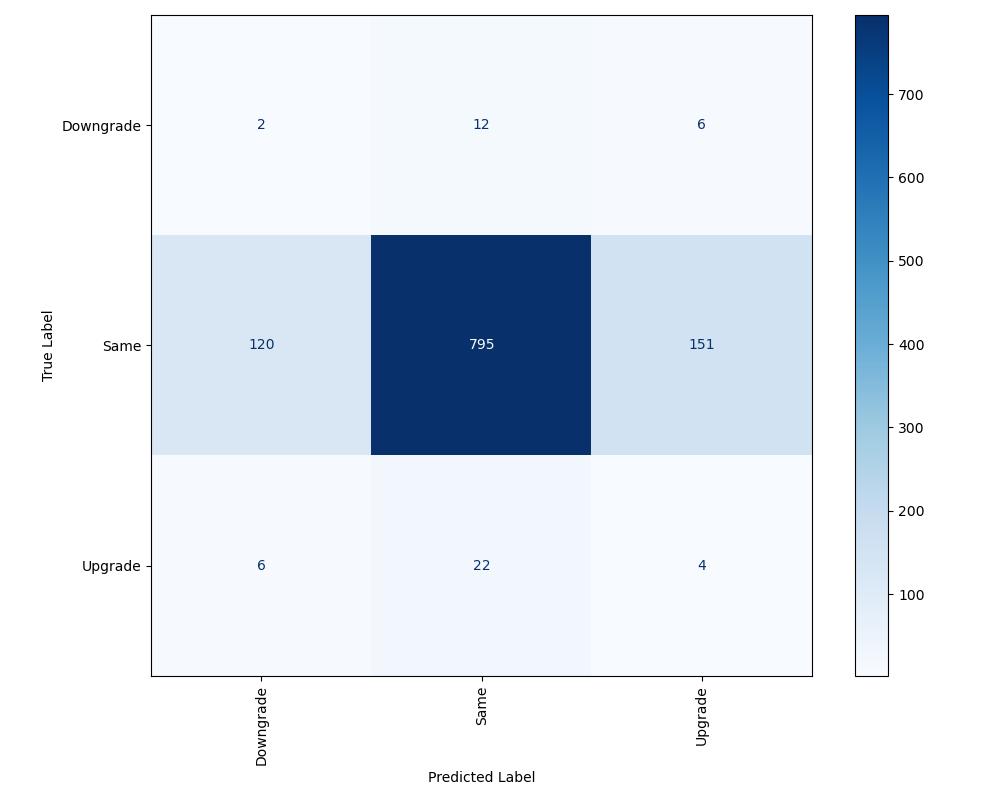
\includegraphics[width=0.95\hsize]{../Output/Modelling/Logistic Regression/smote_rating_change_model_3/smote_rating_change_model_3_confusion_matrix_no_title.png}
            \subcaption*{Logistic Regression}
        \end{subfigure}
        %\hfill
        \begin{subfigure}[h]{0.4925\textwidth}
            \centering
            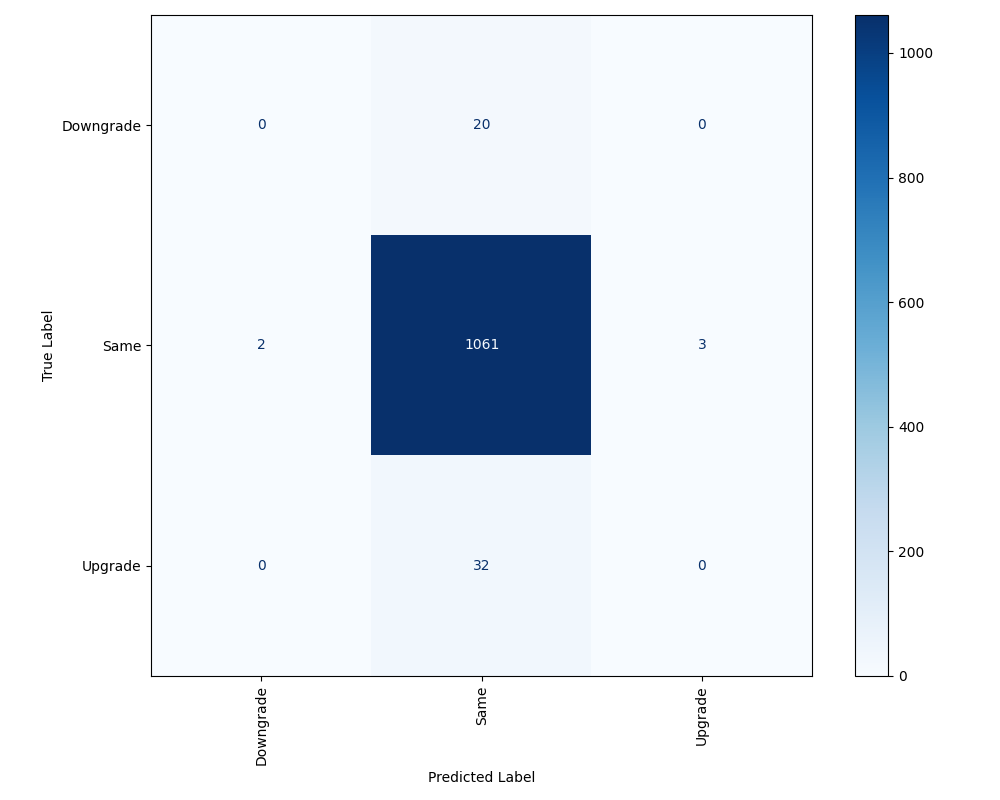
\includegraphics[width=0.95\hsize]{../Output/Modelling/XGBoost/smote_rating_change_model_3/smote_rating_change_model_3_confusion_matrix_no_title.png}
            \subcaption*{XGBoost}
        \end{subfigure}
        \hfill
        \label{fig:change-confusion-matrix}
    \end{figure*}

    \clearpage
    \newpage

    \subsection{McNemar's Test}

    \label{sec:mcnemars-test}

    We make use of McNemar's Test to check for statistically significant differences between our models (usually those without NLP features and including NLP features).

    This test makes use of the following contingency table using counts over observations in our test dataset:

    \begin{center}
        \begin{tabular}{|c|c|c|c|}
            \hline 
                & Model Y Correct & Model Y Incorrect & Row Total\tabularnewline
            \hline 
            \hline 
            Model X Correct & $a$ & $b$ & $a+b$\tabularnewline
            \hline 
            Model X Incorrect & $c$ & $d$ & $c+d$\tabularnewline
            \hline 
            Column Total & $a+c$ & $b+d$ & $n$\tabularnewline
            \hline 
        \end{tabular}
    \par\end{center}

    Under the null hypothesis of identical performance, the marginal probabilities of each model being correct and incorrect are the same: 

    \[
    p_{a}+p_{b}=p_{a}+p_{c}
    \]

    \[
    p_{c}+p_{d}=p_{b}+p_{d}
    \]

    which reduces to

    \[
    H_{0}:p_{b}=p_{c}
    \]

    \[
    H_{1}:p_{b}\neq p_{c}
    \]

    The test statistic is

    \[
    \frac{(b-c)^{2}}{b+c}\sim\chi_{1}^{2}
    \]

    (chi-squared with one degree of freedom) under $H_{0}$, for sufficiently large $b$ and $c$ (heuristically, at least 10 for each). For a derivation (similar to that for the standard Chi-Squared test), see \cite{mcnemar_note_1947} or \cite{rice_mathematical_2006}. We can then compute p-values and assess significance at the 5\% level.

    There are modifications of the test to perform continuity correction, as well as to handle small values of $b+c$ by making it exact with a binomial distribution, but for our purposes these versions always produced the same conclusions regarding significance at 5\%.

    McNemar's test is paired, enabling us to effectively make comparisons between our models when they both face the same observations in the test dataset. At the same time, it operates on counts of the data (our counts correct and incorrect) and is non-parametric, without normality or other distributional assumptions. (Note: the test does still assume independence across observations, but it is difficult to perform testing without this.)

    The results of our tests are shown in Table \ref{tab:p-values} below. p-values are rounded to two decimal places. Items are dashed where there was no difference in accuracy.

    \begin{table*}[h!]
        \centering
        \caption{p-values for McNemar's Test}
        \tiny
\begin{tabular}{ccccc}
\toprule
Model A & Model B & p, Non-Exact & p, Non-Exact, Continuity Corrected & p, Exact \\
\midrule
Logistic - Exclude Previous Rating - Fin Only & Logistic - Exclude Previous Rating - Fin + NLP & 0.31 & 0.35 & 0.35 \\
Logistic - Include Previous Rating - Fin Only & Logistic - Include Previous Rating - Fin + NLP & - & - & - \\
Logistic - SMOTE Rating Change - Fin Only & Logistic - SMOTE Rating Change - Fin + NLP & 0.17 & 0.19 & 0.19 \\
XGBoost - Exclude Previous Rating - Fin Only & XGBoost - Exclude Previous Rating - Fin + NLP & 0.0 & 0.0 & 0.0 \\
XGBoost - Include Previous Rating - Fin Only & XGBoost - Include Previous Rating - Fin + NLP & - & - & - \\
XGBoost - SMOTE Rating Change - Fin Only & XGBoost - SMOTE Rating Change - Fin + NLP & 0.06 & 0.11 & 0.11 \\
GNN - Transductive - Fin + NLP & Logistic Regression - Retrain on GNN Data - Fin + NLP & 0.03 & 0.03 & 0.03 \\
GNN - Transductive - Fin + NLP & Logistic Regression - Pretrained, on GNN Data - Fin + NLP & 0.08 & 0.09 & 0.09 \\
GNN - Transductive - Fin + NLP & XGBoost - Retrain on GNN Data - Fin + NLP & 0.0 & 0.0 & 0.0 \\
GNN - Transductive - Fin + NLP & XGBoost - Pretrained, on GNN Data - Fin + NLP & 0.0 & 0.0 & 0.0 \\
GNN - Transductive - Fin Only & GNN - Transductive - Fin + NLP & 0.17 & 0.21 & 0.21 \\
GNN - Transductive - Fin Only & GNN - Inductive - Fin Only & 0.83 & 0.92 & 0.92 \\
GNN - Transductive - Fin + NLP & GNN - Inductive - Fin + NLP & 0.48 & 0.55 & 0.55 \\
GNN - Inductive - Fin + NLP & Logistic Regression - Retrain on GNN Data - Fin + NLP & 0.01 & 0.01 & 0.01 \\
GNN - Inductive - Fin + NLP & Logistic Regression - Pretrained, on GNN Data - Fin + NLP & 0.03 & 0.04 & 0.04 \\
GNN - Inductive - Fin + NLP & XGBoost - Retrain on GNN Data - Fin + NLP & 0.0 & 0.0 & 0.0 \\
GNN - Inductive - Fin + NLP & XGBoost - Pretrained, on GNN Data - Fin + NLP & 0.0 & 0.0 & 0.0 \\
GNN - Inductive - Fin Only & GNN - Inductive - Fin + NLP & 0.1 & 0.12 & 0.12 \\
\bottomrule
\end{tabular}

\normalsize
        \label{tab:p-values}
    \end{table*}

    \clearpage
    \newpage
    \subsection{Logistic Regression - Most Complex Model - Additional Details}

    \label{sec:logistic-most-complex-model-additional-details}

    Table \ref{tab:logistic-most-complex-classification-report} shows our detailed classification report for our logistic regression model incorporating all of the financial and NLP features. Our use of balanced class weighting enables the model to perform fairly well, even for rare classes.

    \begin{table*}[h!]
        \centering
        \caption{Classification Report - Most Complex Logistic Regression Model}
        \footnotesize
\begin{tabular}{ccccc}
\toprule
Rating & Precision & Recall & F1-Score & Support \\
\midrule
AAA & 0.8261 & 0.7917 & 0.8085 & 24 \\
AA & 0.6316 & 0.6923 & 0.6606 & 52 \\
A & 0.5874 & 0.6298 & 0.6079 & 208 \\
BBB & 0.6909 & 0.6281 & 0.6580 & 363 \\
BB & 0.6275 & 0.5458 & 0.5838 & 284 \\
B & 0.5864 & 0.7273 & 0.6493 & 154 \\
CCC & 0.5556 & 0.7692 & 0.6452 & 26 \\
CC & 0.3333 & 1.0000 & 0.5000 & 2 \\
C & 1.0000 & 1.0000 & 1.0000 & 4 \\
D & 1.0000 & 1.0000 & 1.0000 & 1 \\
\bottomrule
\end{tabular}

\normalsize
        \label{tab:logistic-most-complex-classification-report}
    \end{table*}

    In addition to this, Table \ref{tab:logistic-most-complex-best-params} shows all the optimal hyperparameters we were able to find via grid search. We are able to handle our high-dimensional data with hundreds of variables effectively by using Elastic Net (which collapses to entirely a LASSO penalty) with a slight amount of regularization (C). A one versus rest multiclass prediction setup is used, where a binary is/is not logistic regression probability is estimated for each class, and the class with the highest score is taken.

    \begin{table*}[h!]
        \centering
        \caption{Best Hyperparameters - Most Complex Logistic Regression Model}
        \footnotesize
\begin{tabular}{cccccc}
\toprule
C & Class Weighting Strategy & L1 Ratio & Multi-Class Strategy & Penalty & Solver \\
\midrule
0.10 & Balanced & 1.00 & One vs Rest & Elastic Net & SAGA \\
\bottomrule
\end{tabular}

\normalsize
        \label{tab:logistic-most-complex-best-params}
    \end{table*}

    \clearpage
    \newpage

    \subsection{XGBoost - Most Complex Model - Additional Details}

    \label{sec:xgboost-most-complex-model-additional-details}

    Table \ref{tab:xgboost-most-complex-classification-report} shows our detailed classification report for our XGBoost model incorporating all features. Though we do not use balanced class weighting, recall for small classes is usually very good.

    \begin{table*}[h!]
        \centering
        \caption{Classification Report - Most Complex XGBoost Model}
        \footnotesize
\begin{tabular}{ccccc}
\toprule
Rating & Precision & Recall & F1-Score & Support \\
\midrule
A & 0.8447 & 0.8894 & 0.8665 & 208 \\
AA & 0.8824 & 0.5769 & 0.6977 & 52 \\
AAA & 0.9048 & 0.7917 & 0.8444 & 24 \\
B & 0.9272 & 0.9091 & 0.9180 & 154 \\
BB & 0.9357 & 0.9225 & 0.9291 & 284 \\
BBB & 0.9129 & 0.9532 & 0.9326 & 363 \\
C & 1.0000 & 1.0000 & 1.0000 & 4 \\
CC & 1.0000 & 0.5000 & 0.6667 & 2 \\
CCC & 0.7857 & 0.8462 & 0.8148 & 26 \\
D & 1.0000 & 1.0000 & 1.0000 & 1 \\
\bottomrule
\end{tabular}

\normalsize
        \label{tab:xgboost-most-complex-classification-report}
    \end{table*}

    Table \ref{tab:xgboost-most-complex-best-params} displays the optimal hyperparameters for our XGBoost model incorporating all financial and NLP features. To minimize risk of overfitting, we employed a gamma parameter to control the minimum loss reduction required to make further leaf nodes, in addition to limitations on maximum tree depth and the minimum weight needed to make a further split. We used a fairly high number of estimators to create our predictions.

    \begin{table*}[h!]
        \centering
        \caption{Best Hyperparameters - Most Complex XGBoost Model}
        \footnotesize
\begin{tabular}{ccccc}
\toprule
Gamma & Learning Rate & Max Depth & Min Child Weight & Number of Estimators \\
\midrule
0.10 & 0.10 & 20 & 5 & 1,000 \\
\bottomrule
\end{tabular}

\normalsize
        \label{tab:xgboost-most-complex-best-params}
    \end{table*}

    \clearpage
    \newpage

    \subsection{Graph Neural Network Architecture}

    \label{sec:gnn-architecture}

    % begin lyx insertion

    A GraphSage GCN is trained across a number of timesteps (here indexed by $r$) which progressively mix information from the embeddings of more and more distant neighbors. Creating these embeddings for a given timestep is a two-step process.

    First, in the AGG step, the embeddings of the node's direct neighbors are aggregated. We use what is referred to as pool or pooling aggregation: for node $h$, with neighborhood $N(i)$, at timestep $r$,

    \[
    h_{N(i)}^{(r)}=max[\sigma(W_{pool}h_{j}^{(r-1)}+b),\forall j\in N(i)]
    \]

    meaning the neighboring embeddings from the previous timestep are fed through a fully connected neural network (weights $W_{pool}$, bias $b$, ReLU activation $\sigma)$, and then the elementwise maximum across the new neighbor representations is taken as the aggregated vector.

    Next, during the update (or COMBINE) step, we concatenate the representation of our node of interest from the previous timestep with this aggregated vector, then apply another set of weights and activation (in our case, ReLU again) to get a fully updated node representation.

    \[
    h_{i}^{(r)}=\sigma(W^{(r)}*CONCAT[h_{i}^{(r-1)},h_{N(i)}^{(r)}])
    \]

    The operations for each timestep ultimately represent a layer of the neural network - a SAGEConv layer, of which we have 3. For our classification task, the last of these produces output with dimension of the number of classes (for each node), while we use vectors of size 128 for intermediate $h$ values. Our implementation includes a bias term after the weight application in the update step, and the update step of our last layer does not have an activation function.
    
    Our entire process is trained end-to-end with cross entropy loss for rating classification. We perform weight decay at rate 1e-2, dropout at rate 0.4, and train for 300 epochs at a learning rate of 0.01, using a class stratified 80-20 train-val split and selecting the model state from the epoch with the highest validation accuracy.

    % end lyx insertion

\end{document}
